



Linear algebra is the area of mathematics concerned with \emph{vector spaces} and the \emph{linear maps} between them. On the face of it this sounds like quite a specialised topic, but the truth is quite the opposite -- linearity is everywhere. Whether you are solving simultaneous equations, studying differential equations, working in geometry, or doing quantum mechanics, the underlying structure is frequently that of a vector space, and the machinery developed in this course (bases, matrices, determinants, eigenvalues, inner products and more) is the machinery used to understand it.

This article constitutes my notes for the `Linear Algebra' course, held in Michaelmas 2021 at Cambridge. These notes are \emph{not a transcription of the lectures}, and differ significantly in quite a few areas. Still, all lectured material should be covered. As a warning, this course has lots of results which involve just checking that a definition holds -- such proofs have been intentionally omitted.




\section{Vector Spaces}

\subsection{Vector Spaces and Subspaces}

Linear algebra is, somewhat obviously, primarily about studying objects that are \emph{linear} in nature. The objects we really care about are \emph{vector spaces}, settings in which we can add elements and multiply by scalars. We are also going to consider \emph{linear maps}, functions on vector spaces which preserve that linear structure -- but more on that later. 

Throughout the following discussion (and this course), $\F$ is going to denote an arbitrary field\footnote{A field $\F$ is a set $\F$ equipped with two operations $+$ (`addition') and $\cdot$ (`multiplication'). We require $\F$ with addition to form an abelian group, and multiplication must be associative and have an identity element $1$. We also require every element except $0$ to have an inverse with respect to multiplication, and multiplication must be distributive over addition.

Informally, you can think of a field as something you can do arithmetic in.}

\begin{definition}[$\F$-Vector Space ]
    An \vocab{$\F$-vector space} is an abelian group $(V, +)$ together with a function $\F \times V \rightarrow V$, written $(\lambda, v) \mapsto \lambda v$ such that the following axioms hold:
    \begin{enumerate}[label=(\roman*)]
        \item \emph{Distributivity in $V$}. $\lambda(v_1 + v_2) = \lambda v_1 + \lambda v_2$,
        \item \emph{Distributivity in $\F$}. $(\lambda_1 + \lambda_2)v = \lambda_1 v + \lambda_2 v$,
        \item \emph{Associativity}. $\lambda(\mu v) = (\lambda \mu) v$,
        \item \emph{Identity}. $1v = v$.
    \end{enumerate} 
\end{definition}

We usually call elements of $V$ \vocab{vectors} and elements of $\F$ \vocab{scalars}. The identity element in $V$ is usually called the zero vector, and is written $0_V$ (or just $0$ if the context is clear).

If $\F$ is $\R$ or $\C$, we use the terms `real vector space' and `complex vector space', since they're so common. 


\begin{example}[Examples of Vector Spaces]~
    \vspace{-1.5\baselineskip}
    \begin{enumerate}[label=(\roman*)]
        
        \item The set of triples
        $$
        \{(x, y, z) \mid x, y, z \in \R\}
        $$ 
        forms a real vector space called $\R^3$, because you can add any two triples component wise. 
        \item The set
        $$
        \Q[\sqrt{2}] = \{a + b\sqrt{2} \mid a, b \in \Q\}
        $$
        is a $\Q$-vector space, where we add elements and scale by rational numbers in the obvious way.
        \item The set $\mathcal{C}[0, 1]$ of all continuous functions $f: [0, 1] \rightarrow \R$ forms a real vector space.
    \end{enumerate}
\end{example}

As with many new objects, it's helpful to be able to discuss its substructure. In the case of a vector space $V$, there's a pretty natural notion for what it means for a subset $U \subseteq V$ to still act like a vector space.

\begin{definition}[Subspace]
    Let $V$ be a $\F$-vector space.
    A subset $U \subseteq V$ is a \vocab{subspace} of $V$ if $U$ is also an $\F$-vector space. If $U$ is a subspace of $V$, we will write $U \leq V$.
    
    % \begin{enumerate}[label=(\roman*)]
    %     \item $0 \in U$,
    %     \item $u_1, u_2 \in U$ implies that $u_1 + u_2 \in U$,
    %     \item $\lambda \in \F$, $u \in U$ implies that $\lambda u \in U$.
    % \end{enumerate}
\end{definition}

\begin{example}[Examples of Subspaces]~
    \vspace{-1.5\baselineskip}
    \begin{enumerate}[label=(\roman*)]
        \item The set of vectors $\{(x, y, z) \mid x, y, z \in \R, x + y + z = 0\}$ is a subspace of $\R^3$.
        \item The set of polynomials with terms of even degree $\{ a_0 + a_2 x^2 + a_4 x^4 + \cdots + a_{2k} x^{2k} \mid a_{2i} \in \R, k \in \N\}$ is a subspace of $\R[X]$, the vector space of polynomials with coefficients in $\R$.
    \end{enumerate}
\end{example}

As you would expect, checking that something is a subspace is usually easier than checking all of the axioms for a vector space. In particular, to check that $U$ is a subspace of an $\F$-vector space $V$, you can just check that the following hold:
\begin{itemize}
    \item \emph{Zero vector}\footnote{You may wonder why we need to check this when we already check that we are closed under scaling. To see why, notice that we still have to ensure $U$ is non-empty!}. $0_V \in U$,
    \item \emph{Closure under addition}. $u_1, u_2 \in U$ to imply $u_1 + u_2 \in U$,
    \item \emph{Closure under scaling}. $\lambda \in \F$ and $u \in U$ to imply $\lambda u \in U$.
\end{itemize}


There are various ways in which we can manipulate subspaces, for example we can take the intersection of two subspaces, and we will get back another subspace. 

\begin{proposition}[Intersecting Subspaces]
    Let $U, W \leq V$. Then $U \cap W \leq V$.
\end{proposition}
\begin{proof}
    Since $U$ and $W$ are both subspaces of $V$, we have $0_V \in U \cap W$, and also since they are both closed under addition and scaling, $u_1, u_2 \in U \cap W$ implies that $u_1 + u_2 \in U \cap W$, and $\lambda \in \F$ implies $\lambda u \in U\cap W$. Thus $U \cap W$ is a subspace of $V$. 
\end{proof}

However we can't manipulate subspaces however we want and expect magic. For example, the union of two subspaces is generally \emph{not} a subspace, as it is typically not closed under addition. In fact, the union is only ever a subspace if one of the subspaces is contained in the other.\footnote{There are some more exercises of this flavour on the example sheet.}
You can see what goes wrong already in $\R^2$: if $U$ and $W$ are two distinct lines through the origin, then adding a vector from each takes you off both lines.
\begin{center}
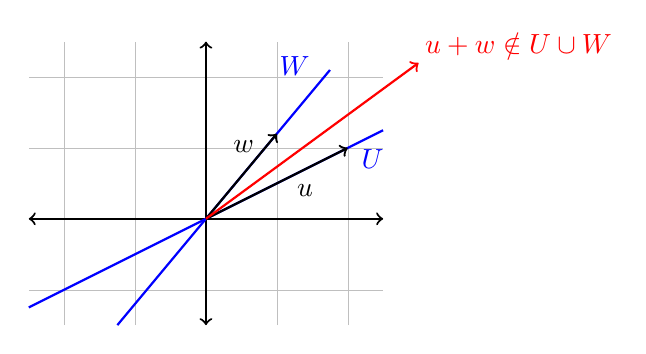
\begin{tikzpicture}[scale=0.9]
    \draw[ultra thin, color=lightgray] (-2.5,-1.5) grid (2.5,2.5);
    \draw[<->] (-2.5,0) -- (2.5,0);
    \draw[<->] (0,-1.5) -- (0,2.5);
    \draw[thick, color=blue] (-2.5,-1.25) -- (2.5,1.25);
    \draw[thick, color=blue] (-1.25,-1.5) -- (1.25*1.4,1.5*1.4);
    \node[color=blue] at (2.35,0.85) {$U$};
    \node[color=blue] at (1.25,2.15) {$W$};
    \draw[->, thick] (0,0) -- (2,1) node[pos=0.7, below, inner sep=5pt] {$u$};
    \draw[->, thick] (0,0) -- (1,1.2) node[pos=0.85, left, inner sep=4pt] {$w$};
    \draw[->, thick, color=red] (0,0) -- (3,2.2) node[above right, inner sep=2pt] {$u + w \notin U \cup W$};
\end{tikzpicture}
\end{center}
We can however try to `complete' the union so that it becomes a subspace.

\begin{definition}[Sum of Subspaces]
    Let $V$ be a vector space over $\F$, and let $U, W \leq V$. We define the \vocab{sum} of $U$ and $W$ to be the set
    $$
    U + W = \{u + w \mid u \in U, w \in W \}.
    $$
\end{definition}

This definition immediately forces $U + W \leq V$, and indeed it is the minimal such space (in that any subspace of $V$ containing both $U$ and $W$ must also contain $U + W$).

\subsection{Quotient Spaces}

Since a vector space $V$ forms an abelian group $(V, +)$, we are able to take the quotient by any subspace $U \leq V$. 

\begin{definition}[Quotient Space]
    Let $V$ an $\F$-vector space, and let $U \leq V$. The \vocab{quotient space} $V/U$ is the abelian group $V/U$ equipped with the scalar multiplication $F \times V/U \rightarrow V/U$ written $(\lambda, v + U) \mapsto \lambda v + U$.
\end{definition}

With this definition, we need to check that this scalar multiplication operation 
is well defined. Indeed, if $v_1 + U = v_2 + U$ then
\begin{align*}
    v_1 - v_2 &\in U \\
\implies \lambda(v_1 - v_2) &\in U \\
\implies \lambda v_1 + U &= \lambda v_2 + U \in V/U,
\end{align*}
so our operation is indeed well defined.

As you would expect, taking a quotient gives you back a vector space.

\begin{proposition}[Quotient Spaces are Vector Spaces]
    $V/U$ is an $\F$-vector space.
\end{proposition}
\begin{proof}[Proof Sketch]
    Check definitions (most properties are inherited from $V$ being a vector space).
\end{proof}

% \subsection{Spans, Linear Independence, and Steinitz Exchange Lemma}

\subsection{Basis and Dimension}

You are likely informally familiar with the idea of \emph{dimension}, a measure how much freedom exists in a system. Dimensionality is a rather natural concept with respect to vector spaces, but we will need to move through some technicalities to establish the results we want.

To discuss the amount of freedom, we first need a way to quantify what it means for a set of vectors to be independent from one another. This is the idea of \emph{linear independence}.


\begin{definition}[Linear Independence]
We say that $\{v_1, \dots, v_n\} \in V$ are \vocab{linearly independent} if
$$
\lambda_1 v_1 + \lambda_2 v_2 + \cdots + \lambda_n v_n = 0
$$
implies that $\lambda_1 = \cdots = \lambda_n = 0$.
\end{definition}

\begin{remark}
    For an infinite subset $S \subseteq V$, we say it's linearly independent if every finite subset is linearly independent.
\end{remark}

If a set of vectors is \emph{not} linearly independent, then there's some vector in that set that can be written as a linear combination of the others -- so it's not independent of them!

The next idea we need to pin down is being able to see if our set of vectors can `generate' the rest of our vector space. 


\begin{definition}[Span]
    Let $V$ be a vector space over $\F$, and let $S \subset V$. We define the \vocab{span} of $S$, $\langle S \rangle$ to be the set of finite combinations of elements of $S$.

    If $\langle S \rangle = V$, then we say $S$ \vocab{spans} or \vocab{generates} $V$.
\end{definition}

\begin{remark}
    By convention, we also take $\langle \emptyset \rangle = \{ 0\}$. An equivalent definition is that $\langle S \rangle$ is the smallest subspace of $V$ that contains $S$.
\end{remark}

\begin{example}[Quadratic Polynomials]
    Let $V$ be the vector space of quadratic polynomials over $\R$, 
    $$V = \{ax^2 + bx + c \mid a, b, c \in \R\}.$$ 
    Then the subset $S \subseteq V$ with $S = \{1, x, x^2\}$ spans $V$.
\end{example}

% \begin{definition}[Finite Dimension]
%     Let $V$ be a vector space over $\F$. We say that $V$ is \vocab{finite dimensional} if it is spanned by a finite set.
% \end{definition}

% \begin{example}[Finite and Infinite Dimensional Vector Spaces]
%     The space $\R[X]$ of polynomials with coefficients in $\R$ is infinite dimensional, but the space $\R_n[X]$ of polynomials of degree at most $n$ is finite dimensional, and is spanned by the set $\{1, X, X^2, \dots, X^n\}$.
% \end{example}

% \begin{definition}[Linear Independence]
% We say that $\{v_1, \dots, v_n\} \in V$ are \vocab{linearly independent} if
% $$
% \lambda_1 v_1 + \lambda_2 v_2 + \cdots + \lambda_n v_n = 0
% $$
% implies that $\lambda_1 = \cdots = \lambda_n = 0$.
% \end{definition}

% If a set of vectors is \emph{not} linearly independent, then one of the vectors in the set can be written as a linear combination of the others. 

% \begin{remark}
%     If $\{v_1, \dots, v_n\}$ are linearly independent, then $v_i \neq 0$ for all $i$.
% \end{remark}

Putting these two concepts together gives us the idea of \emph{bases}, which are sets of linearly independent vectors that span a vector space.

\begin{definition}[Basis]
    A subset $S$ of a vector space $V$ is a \vocab{basis} if $S$ is a set of linearly independent vectors that span $V$.
\end{definition}

\begin{example}[Basis for $\R^n$]
    The \vocab{canonical basis} of $\R^n$ is the set of vectors
    $$
    S = \left\{
        \begin{pmatrix}1 \\ 0 \\ \vdots \\ 0\end{pmatrix},
        \begin{pmatrix}0 \\ 1 \\ \vdots \\ 0\end{pmatrix},
        \dots,
        \begin{pmatrix}0 \\ 0 \\ \vdots \\ 1\end{pmatrix}
    \right\}.
    $$
    Importantly, this is not the \emph{only} basis of $\R^n$, just one that is quite convenient most of the time.
\end{example}

\begin{remark}
    Note that in the definition of a basis there is no requirement for the set of basis vectors $S \subseteq V$ to be finite -- only that any element in $V$ must be representable using finitely many elements of $S$. 
\end{remark}

We'd intuitively want to say that the \emph{dimension} of a vector space is the number of elements in its basis. However, we first need to check that this is a well defined notion.
We can at this point distinguish between finite and infinite dimensional vector spaces at this point though\footnote{Can you see why this is well defined already?}.

\begin{definition}[Finite \& Infinite Dimension]
    We say a vector space $V$ is \vocab{finite dimensional} if it has a finite basis, and we say it is \vocab{infinite dimensional} otherwise.
\end{definition}

The next result about bases we will prove is that they induce \emph{unique} representations of elements in the vector space.

\begin{lemma}[Unique Representations with a Basis]
    Let $V$ be a vector space over $\F$. Then $S \subseteq V$ is a basis of $V$ if and only if any vector $v \in V$ can be written uniquely as a linear combination of elements $v_1, \dots, v_n \in S$.
\end{lemma}
\begin{proof}
    Suppose that $S$ was a basis for $V$.
    Then if $v \in V$ can't be written as such a linear combination, then $S$ wouldn't span $V$, contradicting it being a basis.
    Also, if $v$ can be written as such a linear combination non-uniquely, then taking
    $$
v = \lambda_1 v_1 + \cdots + \lambda_n v_n = \mu_1 v_1 + \cdots + \mu_n v_n.
    $$
    where $\lambda_i \neq \mu_i$ for at least one value of $i$, we'd have
    $0 = v - v = (\lambda_1 - \mu_1) v_1 + \cdots + (\lambda_n - \mu_n)v_n$,
    and at least one of these coefficients must be non-zero, contradicting $S$ being linearly independent.

    Alternatively, if any element in $V$ \emph{can} be written uniquely, then if $v_1, \dots, v_n \in S$ with $\lambda_1 v_1 + \cdots \lambda_n v_n = 0$ implies that $\lambda_1 = \cdots = \lambda_n = 0$, giving that $S$ must be linearly independent. Since $S$ is also spanning by definition, we see that it therefore must be a basis of $V$.
\end{proof}

With that out of the way, we can prove some results about finite dimensional vector spaces which will help us get towards our definition of dimension. 

\begin{lemma}[Spanning Sets Contain a Basis]
    Let $V$ be a finite dimensional vector space, and let $S = \{v_1, \dots, v_n\}$ be a set of vectors that spans $V$. Then there is some subset of $S$ that is a basis of $V$.
\end{lemma}
\begin{proof}
    If $\{v_1, \dots, v_n\}$ is linearly independent, then we are done. If it's not, then (up to reordering) we have $v_n \in \langle\{v_1, \dots, v_{n - 1}\}\rangle$. But then $\langle\{v_1, \dots, v_n\}\rangle = \langle\{v_1, \dots, v_{n - 1}\}\rangle$, so we can not include $v_n$ in our subset. Not including elements in this way repeatedly, since there is finitely many elements in $S$, we must eventually get a linearly independent set that still spans $V$.
\end{proof}

\begin{theorem}[Steinitz Exchange Lemma]
    Let $V$ be a finite dimensional vector space. Then if $\{v_1, \dots, v_m\}$ is a set of linearly independent vectors, and $\{w_1, \dots, w_n\}$ spans $V$, then
    \begin{enumerate}[label=(\roman*)]
        \item $m \leq n$
        \item up to reordering, $\{v_1, \dots, v_m, w_{m + 1}, \dots, w_n\}$ spans $V$.
    \end{enumerate}
\end{theorem}
\begin{proof}
    We will prove this by induction. Suppose we have replaced $\ell \geq 0$ of the $w_i$, and that
    $$
    \langle \{ v_1, \dots, v_\ell, w_{\ell + 1}, \dots, w_n\}\rangle = V.
    $$
    If $m = \ell$, we are done, so assume that $\ell < m$. Then since this set is spanning, we can write $v_{\ell + 1} \in V$ as
    $$
    v_{\ell+1} = \alpha_1 v_1 + \cdots + \alpha_{\ell} v_{\ell} + \beta_{\ell + 1} w_{\ell + 1} + \cdots + \beta_n w_n.
    $$ 
    Since having $\beta_i = 0$ for all $\ell + 1 \leq i \leq n$ would violate linear independence, we can suppose without loss of generality that $\beta_{\ell + 1} \neq 0$. We also note that this implies that $\ell + 1 \leq n$, as otherwise this would not be possible.

    Then $w_{\ell + 1} \in \langle \{v_1, \dots, v_{\ell + 1}, w_{\ell + 2}, \dots, w_{n} \} \rangle$, and this set spans $V$.

    Repeating this process, we will be done after $m$ steps, and we have also shown (at the final step) that $m \leq n$.
\end{proof}

\begin{corollary}[Dimension]
    Let $V$ be a finite dimensional vector space over $\F$. Then any two bases of $V$ have the same number of elements, called the \vocab{dimension} of $V$, denoted $\dim V$ or $\dim_\F V$.
\end{corollary}
\begin{proof}
    Immediate by Steinitz exchange lemma.
\end{proof}

So using Steinitz exchange lemma we have finally been able to pin down exactly what is meant by the dimension of a vector space -- it's the size of it's basis.
This should match up to the intuitive idea of `freedom' that you had at the start of this section. Freedom in a vector space comes from varying coefficients, and in a basis we can both freely vary coefficients and also reach any element in a vector space uniquely, so the number of independent parameters really is the size of the basis.

Steinitz also gives us a few useful results for free.

\begin{corollary}
    Let $V$ be a vector space over $\F$ with finite dimension $n = \dim V$. Then
    \begin{enumerate}[label=(\roman*)]
        \item Any independent set of vectors has at most $n$ elements, with equality if and only if it's a basis.
        \item Any spanning set has at least $n$ elements, with equality if and only if it's a basis.
    \end{enumerate} 
\end{corollary}
\begin{proof}
    Immediate by Steinitz exchange lemma.
\end{proof}

Working with basis and dimension can make the study of vector spaces much easier. For example, Steinitz allows us nicely extend bases. That is,
\begin{center}
	\color{blue}
    If we have a vector space $V$, and a subspace $U \leq V$, \\then we can pick a nice basis $\{u_1, \dots, u_\ell\}$ of $U$, and \\extend it to a basis $\{u_1, \dots, u_{\ell}, u_{\ell + 1}, \dots, u_n\}$ of $V$.
\end{center}Working with ideas like this can make many results easier to prove, as we will see in the following propositions.


\begin{proposition}[Dimension of the Sum of Subspaces]
    Let $U$, $W$ be subspaces of a vector space $V$. If $U$ and $W$ are finite dimensional, then so is $U + W$, and $\dim (U + W) = \dim U + \dim W - \dim (U \cap W)$.
\end{proposition}
\begin{proof}
    Pick a basis $\{v_1, \dots, v_a\}$ of $U \cap W$, and extend by Steinitz exchange lemma to a basis $\{v_1, \dots, v_a, u_1, \dots, u_b\}$ of $U$, and to a basis $\{v_1, \dots, v_a, w_1, \dots, w_c\}$ of $W$.
    
    It suffices to prove that $\{v_1, \dots, v_a, u_1, \dots, u_b, w_1, \dots, w_c\}$ is a basis of $U + W$.

    Clearly this set of vectors spans $U + W$, so we just need to check that they are linearly independent. Suppose that
    $$
    \sum_{i = 1}^{a} \alpha_i v_i + \sum_{i = 1}^b \beta_i u_i + \sum_{i = 1}^c \gamma_i w_i = 0.
    $$
    Rewriting,
    \begin{equation}\label{eq:thing}
        \sum_{i = 1}^{a} \alpha_i v_i + \sum_{i = 1}^b \beta_i u_i = -\sum_{i = 1}^c \gamma_i w_i, \tag{$\dagger$}
    \end{equation}
    where the LHS is in $U$ and the RHS is in $W$. This implies that
    $
    \sum_{i = 1}^c \gamma_i w_i \in U \cap W,
    $
    and can be written as 
    $
    \sum_{i = 1}^c \gamma_i w_i = \sum_{i = 1}^a  \mu_i v_i$,
    for some $\mu_i$, and then substituting this back into \eqref{eq:thing},
    $$
    \sum_{i = 1}^a (\alpha_i + \mu_i) v_i + \sum_{i = 1}^b \beta_i u_i = 0
    $$
    which forces $\beta_i = 0$. A similar argument also gives $\gamma_i = 0$, which then finally forces $\alpha_i = 0$, since $\{v_1, \dots, v_a\}$ is a basis.
\end{proof}

\begin{proposition}[Dimension of the Quotient Space]
    If $V$ is a finite dimensional vector space over $\F$ and $U \leq V$, then $U$ and $V / U$ are also finite dimensional, and $\dim V = \dim U + \dim V / U$.
\end{proposition}
\begin{proof}
    Let $\{u_1, \dots, u_\ell\}$ be a basis of $U$, and extend it via Steinitz exchange lemma to a basis $\{u_1, \dots, u_\ell, w_{\ell+1}, \dots, w_n\}$ of $V$.

    It's easy to see that $\{w_{\ell + 1} + U, \dots, w_{n} + U\}$ is a basis of $V/U$, as it clearly spans and linear independence is inherited from it being a basis of $V$. The result then follows.
\end{proof}

\subsection{Direct Sums}

Previously, we were able to look at the substructure of a vector space by looking at subspaces. Given two subspaces, we were then able to construct their sum, which is the set of all linear combinations of elements in each subspace. 

When studying a vector space using its subspaces in this way (considering their sum), it can be useful to impose an \emph{additional} constraint about the way in which the subspaces interact. In particular, it can be useful to impose a uniqueness constraint on the linear combinations that are created.

\begin{definition}[Direct Sum]
    Let $V$ be a vector space over $\F$, and let $U, W \leq V$. We say that $V$ is the \vocab{direct sum} of $U$ and $W$, written $V = U \oplus W$ if and only if every element $v \in V$ can be decomposed as
    $$
    v = u + w
    $$
    with $u \in U$ and $w \in W$, with this decomposition being unique.
\end{definition}

Of course, we can generalize the notion of a direct sum naturally to the case of multiple subspaces, in the way that you would expect.

\begin{remark}[Warning]
    We say that $W$ is \emph{a} direct complement of $U$ in $V$. There is \emph{no uniqueness} of such a complement!
\end{remark}



\begin{lemma}
    Let $V$ be a vector space and let $U, W \leq V$.
    Then the following are equivalent.
    \begin{enumerate}[label=(\roman*)]
        \item $V = U \oplus W$
        \item $V = U + W$ and $U \cap W = \{0\}$
        \item For any basis $B_1$ of $U$ and $B_2$ of $W$, the union $B = B_1 \cup B_2$ is a basis of $V$.
    \end{enumerate}
\end{lemma}
\begin{proof}
    \emph{(ii) implies (i)}. Let $V = U + W$ with $U \cap W = \{0\}$. Then for all $v \in V$, we can write $v = u + w$ with $u \in U$ and $w \in W$. To see that this is unique, suppose that
    $$
    v = u + w = u' + w'.
    $$
    Then $(u - u') = - (w-w')$, and thus they are both in $U \cap W$, but the only element of this is $0$, and thus $u = u'$ and $w = w'$, giving us uniqueness.

    \emph{(i) implies (iii)}. Let $B_1$ be a basis of $U$ and $B_2$ be a basis of $W$. Then $B = B_1 \cup B_2$ clearly spans $V$, so we need to check that it's linearly independent. Indeed, if
    $$
    \sum_{u \in B_1} \lambda_u u + \sum_{w \in B_2} \lambda_w w = 0,
    $$
    then $V = U \oplus W$ implies that since this is the sum of an element of $U$ and an element of $W$, then each is zero, and linear independence follows from $B_1, B_2$ being sets of linearly independent vectors.

    \emph{(iii) implies (ii)}. 
    Clearly we have $V = U+W$, so we just need to check that $U \cap W = \{0\}$. Let $v \in U \cap W$. Then we can write
    $$
    v = \sum_{u \in B_1} \lambda_u u = \sum_{w \in B_2} \lambda_w w \implies \sum_{u \in B_1} \lambda_u u - \sum_{w \in B_2} \lambda_w W = 0,
    $$
    and since $B_1 \cup B_2$ is a basis for $V$, we must have $\lambda_u, \lambda_w = 0$ for all $u, w \in B_1, B_2$, implying that $v = 0$.
\end{proof}

This result extends as you would expect for the case of direct products using multiple subspaces.

\section{Linear Maps}

\subsection{Linear Maps and Isomorphisms}

We are now going to turn our attention to \emph{linear maps}, which are maps that preserve the underlying structure of the vector space that they act on.

\begin{definition}[Linear Map]
    Let $V, W$ are vector spaces over $\F$.
    A map $\alpha: V \rightarrow W$ is a \vocab{linear map} if for all $\lambda_1, \lambda_2 \in \F$ and $v_1, v_2 \in V$ we have 
    $$
    \alpha(\lambda_1 v_1 + \lambda_2 v_2) = \lambda_1\alpha(v_1) + \lambda_2 \alpha(v_2).
    $$
\end{definition}

\begin{example}[Examples of Linear Maps]~
    \vspace{-1.5\baselineskip}
    \begin{enumerate}[label=(\roman*)]
        \item Consider the vector space $\mathcal{C}[0, 1]$ of continuous functions $f:[0, 1] \rightarrow \R$, Then for any fixed point $x \in [0, 1]$, the map $\alpha: C[0, 1] \rightarrow \R$ with $\alpha(f) = f(x)$ is a linear map.
        \item The map $\R^3 \rightarrow \R$ given by $(a, b, c) \mapsto 4a + 2b + c$ is a linear map.
        \item The map $\alpha: Q[\sqrt{2}] \rightarrow Q[\sqrt{2}]$ of `multiplying by $\sqrt{2}$' is a linear map, with $a + b \sqrt{2} \mapsto 2b + a \sqrt{2}$.
    \end{enumerate}
\end{example}

It's easy to see that the identity map is a linear map, and also that linearity is preserved by composing linear maps.

One nice thing about linear maps is that they interact well with basis, because of linearity. Indeed, specifying a linear map on the basis is sufficient to define that map on all of a vector space.

\begin{lemma}[Extension by Linearity]\label{lemma:extend-map}
    Let $V$ and $W$ be vector spaces, and let $B$ be a basis for $V$. Then if $\alpha_0: B \rightarrow W$ is \emph{any} map, then there exists a \emph{unique} linear map $\alpha: V \rightarrow W$ extending $\alpha_0$, so that for all $v \in B$ we have $\alpha(v) = \alpha_0(v)$.
\end{lemma}
\begin{proof}
    For $v \in V$, let $v = \sum_{i = 1}^n \lambda_i v_i$. Then necessarily by linearity, we define
    $$
    \alpha(v) = \alpha\left(\sum_{i = 1}^n \lambda_i v_i\right) = \sum_{i = 1}^n \lambda_i \alpha_0 (v_i).
    $$
    By construction this is a linear map and it extends $\alpha_0$.
\end{proof}

As with many other areas of pure mathematics, we have a special case for the structure preserving bijections on a given object.

\begin{definition}[Isomorphism]
    If $V$ and $W$ are vector spaces over $\F$, the linear map $\alpha: V \rightarrow W$ is an \vocab{isomorphism} if it also bijective. We say two vector spaces $V$ and $W$ are \vocab{isomorphic}, written $V \cong W$, if there is an isomorphism between them.
\end{definition}

\begin{remark}
    if $\alpha:V \rightarrow W$ is an isomorphism, then the inverse map $\alpha^{-1}$ exists and importantly it's \emph{also} linear.
\end{remark}

\begin{lemma}[Isomorphism is an Equivalence Relation]
    $\cong$ is an equivalence relation on the class of all vector spaces over $\F$.
\end{lemma}
\begin{proof}
    For reflexivity, we note that the identity map $id: V \rightarrow V$ is an isomorphism. For symmetry, we note that if $\alpha: V \rightarrow W$ is an isomorphism, then $\alpha^{-1}: W \rightarrow V$ is also an isomorphism. Lastly, we get transitivity because if $\alpha: U \rightarrow V$ and $\beta: V \rightarrow W$ are isomorphisms, then $\beta \circ \alpha: U \rightarrow W$ is also an isomorphism.
\end{proof}

From one perspective, isomorphism allows us to know when two objects are really just different representations of the same thing. With this in mind, the following result tells us something interesting (yet unsurprising) about the nature of finite dimensional vector spaces.


\begin{theorem}[Isomorphism for Finite Dimensional Vector Spaces]
    If $V$ is an $n$ dimensional vector space over $\F$, then $V \cong \F^n$, the vector space
    $$
    \F^n = \left\{\begin{pmatrix}x_1 \\ x_2 \\ \vdots \\ x_n\end{pmatrix} \mid x_1, \dots, x_n \in \F \right\},
    $$
    where addition is component-wise.
\end{theorem}
\begin{proof}
    Let $B = \{v_1, \dots, v_n\}$ be a basis for $V$. Then we claim that the map $\alpha: V \rightarrow \F^n$ defined by 
    $$
    v = \sum_{i = 1}^n \lambda_i v_i \longmapsto \begin{pmatrix}\lambda_1 \\ \vdots \\ \lambda_n\end{pmatrix}
    $$
    is an isomorphism. Indeed, it's easy to see that we have linearity inherited from $\F$, and also the map is a bijection, so indeed we do have $V \cong \F^n$.
\end{proof}

In particular, this result tells us that when we choose a basis for a finite dimensional vector space $V$, it's really the same as picking some isomorphism from $V$ to $\F^n$. 

This theorem also directly implies (with isomorphism being an equivalence relation) a criterion for two finite dimensional vector spaces to be isomorphic.

\begin{theorem}[Isomorphism Criterion]
    Let $V$ and $W$ be finite dimensional vector spaces over $\F$. Then they are isomorphic if and only if they have the same dimension.
\end{theorem}

\subsection{Images and Kernels}

Stepping back from isomorphisms, we need to define some frequently used concepts relating to linear maps.

\begin{definition}
    Let $V, W$ be vector spaces over $F$, and let $\alpha: V \rightarrow W$ be a linear map. We define the \vocab{kernel} of $\alpha$ as
    $$
    \kernel \alpha = \{ v\in V \mid \alpha(v) = 0\},
    $$
    and the \vocab{image} of $\alpha$ as
    $$
    \image \alpha = \{ w \in W \mid w = \alpha(v), v \in V\}.
    $$
\end{definition}

The structure of a linear map carries over to the image and the kernel, and naturally implies that they are both subspaces of their parent vector spaces.

\begin{lemma}[Image and Kernel are Subspaces]
    Let $\alpha: V \rightarrow W$ be a linear map. Then $\kernel \alpha$ and $\image \alpha$ are subspaces of $V$ and $W$ respectively.
\end{lemma}
\begin{proof}[Proof Sketch]
    Check definitions.
\end{proof}

You may recognize the definitions of the kernel and image from a course in group theory, particularly in relation to the first isomorphism theorem\footnote{Recall that if $G$ and $H$ are groups, and $\phi: G \rightarrow H$ is a homomorphism, then $G/\kernel{\phi} \cong \image \phi$.}. Indeed, remembering that vector spaces with vector addition are groups, with we can use the kernel and image of a linear map to establish an isomorphism between vector spaces.

\begin{theorem}[First Isomorphism Theorem For Vector Spaces]
    Let $V$ and $W$ be $\F$ vector spaces, and let $\alpha: V \rightarrow W$ be a linear map. Then $V/\kernel \alpha \cong \image \alpha$.
\end{theorem}
\begin{proof}[Proof Sketch]
    Consider the isomorphism $\overline{\alpha} : V/\kernel \alpha \rightarrow \image \alpha$ defined by $\overline{\alpha}(v + \kernel \alpha) = \alpha(v)$, and check definitions.
\end{proof}

Now while the kernel and image being subspaces are rather straightforward, slightly more interesting is the \emph{dimension} of these subspaces. This is described by the \emph{rank-nullity theorem}.

\begin{definition}[Rank and Nullity]
    Let $\alpha$ be a linear map. Then the \vocab{rank} of $\alpha$, $r(\alpha) = \dim \image \alpha$, is the dimension of the image. The \vocab{nullity} of $\alpha$, $n(\alpha) = \dim \kernel \alpha$, is the dimension of the Kernel.
\end{definition}

\begin{theorem}[Rank-Nullity Theorem]
    Let $U$ and $V$ be vector spaces such that $U$ is finite dimensional.
    Let $\alpha: U \rightarrow V$ be a linear map. Then
    $$
    \dim U = r(\alpha) + n(\alpha).
    $$
\end{theorem}
\begin{proof}
    We know that $U/\kernel \alpha \cong \image \alpha$. Thus $\dim (U / \kernel \alpha) = \dim (\image \alpha)$, that is $\dim U - \dim \kernel \alpha = \dim \image \alpha$, or $\dim U = r(\alpha) + n(\alpha)$.
\end{proof}

It is worth pausing to picture what this theorem is saying. A linear map $\alpha: U \rightarrow V$ crushes the kernel down to the single point $0$, and maps what remains onto the image inside $V$. The theorem says that the dimensions `lost' and `kept' in this process must account for all of $\dim U$.
\begin{center}
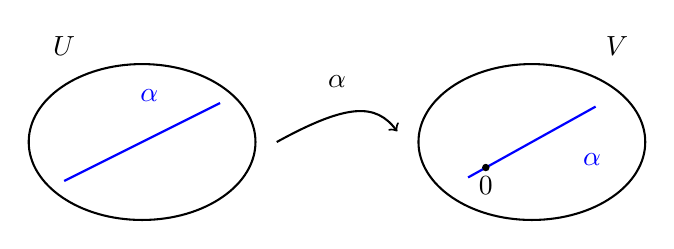
\begin{tikzpicture}[scale=0.9]
    % Domain blob
    \draw (0,0) ellipse (1.6 and 1.1);
    \node at (-1.1,1.35) {$U$};
    % kernel line inside domain
    \draw[thick, color=blue] (-1.1,-0.55) -- (1.1,0.55);
    \node[color=blue] at (0.1,0.65) {$\kernel \alpha$};
    % codomain blob
    \draw (5.5,0) ellipse (1.6 and 1.1);
    \node at (6.7,1.35) {$V$};
    % image inside codomain
    \draw[thick, color=blue] (4.6,-0.5) -- (6.4,0.5);
    \node[color=blue] at (6.35,-0.25) {$\image \alpha$};
    % zero point
    \fill (4.85,-0.36) circle (1.5pt);
    \node[below, inner sep=3pt] at (4.85,-0.36) {$0$};
    % map arrow
    \draw[->] (1.9,0) .. controls (2.9,0.55) and (3.3,0.55) .. (3.6,0.15);
    \node at (2.75,0.85) {$\alpha$};
\end{tikzpicture}
\end{center}
This result has an important consequence which is incredibly useful for quickly checking if a map is an isomorphism.

\begin{lemma}[Characterisation of Isomorphism]
    Let $V$ and $W$ be vector spaces over $\F$ with \emph{equal finite dimension}. Then the following are equivalent: 
    \begin{enumerate}[label=(\roman*)]
        \item $\alpha$ is injective,
        \item $\alpha$ is surjective,
        \item $\alpha$ is an isomorphism.
    \end{enumerate}
\end{lemma}
\begin{proof}[Proof Sketch]
    Follows directly from the rank-nullity theorem.
\end{proof}

\subsection{Matrices}

When dealing with vector spaces, it's sometimes convenient to work with vector spaces in the abstract, and other times it's convenient to pick some nice basis which you can easily work with.
When dealing with linear maps $\alpha: V \rightarrow W$, it it can also be useful to work with bases. The way we do this is by introducing \emph{matrices}.

It's important to say that matrices are not the essence of linear algebra, and in may cases viewing the subject in this way will just give you the impression that linear algebra is an opaque subject. Instead, you should think of matrices as a nice representations of linear maps for which its easy to perform computations with.
With that said, let's talk about linear maps.

In this section, we are going to discuss linear maps between two vector spaces $V$ and $W$.

\begin{definition}[Space of Linear Maps]
    Let $V$ and $W$ be vector spaces over $\F$. We define
    $$
    \mathcal{L}(V, W) = \{\alpha: V \rightarrow W \mid \alpha \text{ is a linear map}\}.
    $$
\end{definition}

\begin{proposition}[Space of Linear Maps is a Vector Space]
    $\mathcal{L}(V, W)$ is a vector space over $\F$. Moreover, if $V$ and $W$ are finite dimensional, then
    $$
    \dim \mathcal{L}(V, W) = \dim V \cdot \dim W.
    $$
\end{proposition}
\begin{proof}[Proof Sketch]    
    To see that $\mathcal{L}(V, W)$ is a vector space, one just needs to check definitions. We will leave the proof of the dimension until later.
\end{proof}

Now, given some linear map $\alpha$, let's think about how we can represent this map with respect to a basis.
Suppose that we had a finite dimensional vector space $V$ with basis $\{v_1, \dots, v_m\}$, and a finite dimensional vector space $W$ with basis $\{w_1, \dots, w_n\}$, and suppose that we had some linear map $\alpha : V \rightarrow W$.

Given some $v \in V$, if we wanted to work out $\alpha(v)$, we can write express $v$ in the basis above, with
$$
\alpha(v) = \alpha\left(\sum_{i = 1}^m \lambda_i v_i\right) = \sum_{i = 1}^m \lambda_i \alpha(v_i).
$$
So, to compute what $\alpha(v)$ is for any $v \in V$, it suffices to know what $\alpha(v_1), \dots, \alpha(v_m)$ is. To specify what say $\alpha(v_1)$ is, we can use the above basis of $W$ and write
$$
\alpha(v_1) = a_{11} w_1 + a_{21} w_2 + \cdots + a_{n1} w_n,
$$
for some coefficients $a_{i1}$. Repeating this for $v_2, \dots, v_n$ then totally specifies the linear map $\alpha$.
These collection of coefficients can be put into a \emph{matrix}, which will then be a representation of $\alpha$ when coupled with the bases $\{v_i\}$ and $\{w_i\}$.


\begin{definition}[Matrix]
    An $n \times m$ \vocab{matrix} over $\F$ is an array with $n$ rows and $m$ columns, with entries in $\F$:
    $$
    A = \begin{pmatrix}
        a_{11} & a_{12} & \cdots & a_{1m} \\
        a_{21} & a_{22} & \cdots & a_{2m} \\
        \vdots&\vdots&\ddots &\vdots\\
        a_{n1} & a_{n2} & \cdots & a_{nm}
    \end{pmatrix}.
    $$
    We denote the set of $n \times m$ matrices over $\F$ by $\mathcal{M}_{n,m}(\F)$.
\end{definition}

\begin{proposition}[Vector Space of Matrices]
    $\mathcal{M}_{n, m}(\F)$ is an $\F$-vector space.
\end{proposition}
\begin{proof}[Proof Sketch]
    Taking addition entry-wise we can just check definitions.
\end{proof}

\begin{proposition}[Dimension of $\mathcal{M}_{n,m}(\F)$]
    $\dim \mathcal{M}_{m, n}(\F) = m \times n$.
\end{proposition}
\begin{proof}
    We define the \emph{elementary matrix} $E_{i, j}$ such that every entry is $0$ except for the $i, j$th entry, which is $1$.
    Then the set $\{E_{i, j} \mid 1 \leq i \leq m, 1 \leq j \leq n\}$ is clearly a basis, and has $n \times m$ elements.
\end{proof}

Following on from the discussion above, we can now write down how linear maps can be represented using matrices.

\begin{definition}[Matrix of $\alpha$ in the $B, C$ Basis]
    Let $\alpha: V \rightarrow W$ be a linear map, and let $B = \{v_1, \dots, v_m\}$ be a basis of $V$ and $C = \{w_1, \dots, w_n\}$ be a basis of $W$. Then we define the \vocab{matrix of $\alpha$} to be
    $$
    [\alpha]_{B, C} = \begin{pmatrix}
        | & | & & | \\
        [\alpha(v_1)]_C & [\alpha(v_2)]_C & \cdots & [\alpha(v_m)]_C \\
        | & | & & |
    \end{pmatrix} = \begin{pmatrix}
        a_{11} & a_{12} & \cdots & a_{1m} \\
        a_{21} & a_{22} & \cdots & a_{2m} \\
        \vdots&\vdots&\ddots &\vdots\\
        a_{n1} & a_{n2} & \cdots & a_{nm}
    \end{pmatrix},
    $$
    where $a_{ij}$ is the coefficient of $w_i$ in $\alpha(v_j)$.
\end{definition}
\begin{remark}[Notation]
    We use $[v]_C$ to denote the column vector representing the vector $v$ in the basis $C$.
\end{remark}


\begin{proposition}[Matrix Representation of Linear Maps]
    If $V$ and $W$ are vector spaces over $\F$ such that $\dim V = n$ and $\dim W = m$, then $\mathcal{L}(V, W) \cong \mathcal{M}_{m, n}(\F)$.
\end{proposition}
\begin{proof}
    Fix a basis $B, C$ of $V$ and $W$ respectively.
    Then consider the linear map
    $
    \theta: \mathcal{L}(V, W) \rightarrow \mathcal{M}_{m, n}(\F)
    $ given by $\alpha \mapsto [\alpha]_{B, C}$.

    This map is clearly linear, and it's also clearly a bijection thus it's an isomorphism and our result follows.
\end{proof}

\begin{remark}
    This implies that $\dim \mathcal{L}(V, W) = m \times n$, filling in the gap left in the proposition at the start of this section.
\end{remark}


What's nice about matrices is that they make working with linear maps \emph{easy}. It's generally much easier to manipulate arbitrary matrices than it is to arbitrary linear maps (of course, this varies from case to case), and we will see this in the following set of computational results.

You should be familiar from previous courses with the notion of matrix multiplication.

\begin{definition}[Matrix Multiplication]
    Let $A = (a_{ij})$ be an $n \times p$ matrix, and $B = (b_{ij})$ 
    be an $p \times m$ matrix.
    Then their \vocab{product} $C = A\cdot B$ is an $n \times m$ matrix $C = (c_{ij})$, with
    $$
    c_{ij} = \sum_{k = 1}^p a_{ik}b_{kj}.
    $$
\end{definition}

We can use matrix multiplication in lots of nice ways.

\begin{lemma}[Evaluating Linear Maps]
    Let $\alpha: V \rightarrow W$ be a linear map, and let $B, C$ be bases for $V$ and $W$ respectively. Then if $v \in V$, we have
    $$
    [\alpha(v)]_C = [\alpha_{B,C}] \cdot [v]_B.
    $$
\end{lemma}
\begin{proof}
    Let $v \in V$, and let $v = \sum_{j = 1}^n \lambda_j v_j$. Then
    $$
    \alpha(v) = \sum_{j = 1}^n \lambda_j \alpha(v_j) = \sum_{j = 1}^n \lambda_j \sum_{i = 1}^m a_{ij} w_i = \sum_{i = 1}^m \left(\sum_{j = 1}^n a_{ij} \lambda_j\right) w_i,
    $$
    as required.
\end{proof}

\begin{lemma}[Composing Linear Maps]
    Let $\alpha: V \rightarrow W$ and $\beta: U \rightarrow V$ be linear maps. Then if $A, B, C$ are bases of $U, V$ and $W$ respectively, we have 
    $$
    [\alpha \circ \beta]_{A, C} = [\alpha]_{B, C} \cdot [\beta]_{A, B}.
    $$
\end{lemma}
\begin{proof}[Proof Sketch]
    Use the definition of matrix multiplication to check that this map corresponds to the correct thing.
\end{proof}


% \begin{example}
%     Let $V$ and $W$ be finite dimensional vector spaces.
%     Consider the linear map $\alpha: V \rightarrow W$, and suppose $Y \leq V$. Consider the image of $Y$ under $\alpha$, $\alpha(Y) = \{ \omega \in W \mid \omega = \alpha(y), y \in Y\}$.

%     Define the sets $B' = \{v_1, \dots, v_k\}$ and $B'' = \{v_{k + 1}, \dots, v_n\}$ such that the union of disjoint sets $B = B' \cup B''$ is a basis for $V$, and $B'$ is a basis of $Y$ (that is, we extend using Steinitz exchange lemma).
    
%     Similarity we define $C' = \{w_1, \dots, w_\ell\}$ and $C'' = \{w_{\ell + 1}, \dots, w_m\}$ such that the union of disjoint sets $C = C' \cup C''$ is a basis for $W$ and $C'$ is a basis for $\alpha(Y)$.

%     Then we have the matrix
%     $$ 
%     [\alpha]_{B, C} = \begin{pmatrix}
%         \alpha(v_1) & \cdots & \alpha(v_k) & \alpha(v_{k + 1}) & \cdots & \alpha(v_n)
%     \end{pmatrix},
%     $$
%     and this will look like the block matrix
%     $$
%     \left[\begin{array}{ c | c }
%         A & B \\
%         \hline
%         0 & C
%       \end{array}\right],
%     $$
%     where $A$ is $k \times \ell$.
% \end{example}

\subsection{Change of Basis and Equivalent Matrices}

Matrices represent a linear map with respect to a given basis, so a natural question is how do we rewrite a matrix in a different basis? That is, 
given two vector spaces $V, W$ and a linear map $\alpha: V \rightarrow W$, we want to take the matrix $[\alpha]_{B, C}$ and express it with respect to the basis $B', C'$. 

The way we do this is by introducing a \emph{change of basis} matrix.

\begin{definition}[Change of Basis Matrix]    
    The \vocab{change of basis} matrix from $B'$ to $B$ is the matrix
    $P = [I]_{B', B}$, where $I$ is the identity map.
\end{definition}
\begin{remark}
    $P$ is an invertible square matrix, and $P^{-1}$ is the change of basis matrix from $B$ to $B'$. 
\end{remark}

Given a vector represented in a basis $B$, the change of basis matrix allows that vector to be expressed in a different basis $B'$.

\begin{lemma}[Change of Basis for a Vector]
    Let $B$ and $B'$ be bases for a vector space $V$, and let $v \in V$. Then if $P$ is the change of basis matrix from $B'$ to $B$ we have
    $$
    [v]_{B} = P[v]_{B'}.
    $$
\end{lemma}
\begin{proof}
    We know that $P = [I]_{B', B}$, and so $[v]_B = [I(v)]_B = [I]_{B', B} [v]_{B'} = P[v]_{B'}$.
\end{proof}

Using this idea of change of basis matrices, we can express the matrix of a linear map with respect to another basis. The situation to keep in mind is the following square, where the vertical arrows are the identity map expressed in the relevant bases -- the two ways of travelling from the top-left corner to the bottom-right corner must agree.
\begin{center}
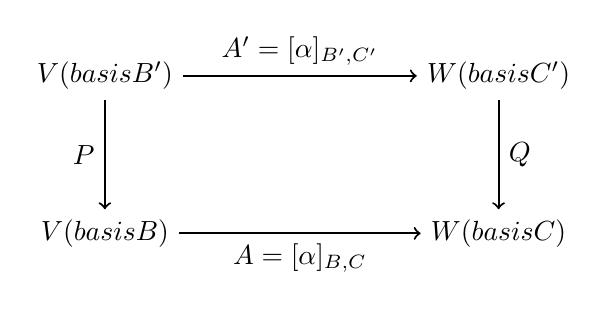
\begin{tikzpicture}[scale=1.0]
    \node (VB') at (0,2) {$V \text{ (basis } B')$};
    \node (WC') at (5,2) {$W \text{ (basis } C')$};
    \node (VB) at (0,0) {$V \text{ (basis } B)$};
    \node (WC) at (5,0) {$W \text{ (basis } C)$};
    \draw[->] (VB') -- (WC') node[midway, above] {$A' = [\alpha]_{B', C'}$};
    \draw[->] (VB) -- (WC) node[midway, below] {$A = [\alpha]_{B, C}$};
    \draw[->] (VB') -- (VB) node[midway, left] {$P$};
    \draw[->] (WC') -- (WC) node[midway, right] {$Q$};
\end{tikzpicture}
\end{center}

\begin{proposition}[Change of Basis Formula]
    Let $A = [\alpha]_{B, C}$ and $A' = [\alpha]_{B', C'}$, and let $P$ be the change of basis from $B'$ to $B$ and $Q$ be the change of basis matrix from $C'$ to $C$. Then
    $$
    A' = Q^{-1} AP.
    $$
\end{proposition}
\begin{proof}
    For any $v \in V$ we have, using the change of basis lemma for vectors twice,
    $$
    Q [\alpha(v)]_{C'} = [\alpha(v)]_C = A [v]_B = AP[v]_{B'},
    $$
    and so $[\alpha(v)]_{C'} = Q^{-1}AP [v]_{B'}$. Since the matrix representing $\alpha$ with respect to $B'$ and $C'$ is unique, $A' = Q^{-1}AP$.
\end{proof}

\subsection{Equivalent Matrices}

A natural notion of equivalence comes from saying 
two matrices are equivalent if there is some choice of basis for which they represent the same linear map. Using the change of basis formula, we can pin down this notion exactly.

\begin{definition}[Equivalent Matrices]
    We say that two matrices $A, A' \in \mathcal{M}_{m, n}(\FF)$ are \vocab{equivalent} if $A' = Q^{-1}AP$ for some invertible matrices $Q \in \mathcal{M}_{m, m}(\F)$ and $P \in \mathcal{M}_{n, n}$.    
\end{definition}

It's easy to check that this definition gives us an equivalence relation, and indeed it turns out that the equivalence classes of matrices are remarkably straightforward.

\begin{proposition}[Natural Basis for Matrices]
    Let $V, W$ be vector spaces over $\F$, with $\dim V = n$ and $\dim W = m$. Let $\alpha: V \rightarrow W$ be a linear map, Then there exists a basis $B$ of $V$ and a basis $C$ of $W$ such that
    $$
    [\alpha]_{B, C} = \left(\begin{array}{ c | c }
        I_r & 0 \\
        \hline
        0 & 0
      \end{array}\right),
    $$
    where $r = r(\alpha)$ and $I_r$ is the $r \times r$ identity matrix.
\end{proposition}
\begin{proof}
    We first choose a basis $\{v_{r + 1}, \dots, v_n\}$ of $\kernel \alpha$, and extend it to a basis $B = \{v_1, \dots, v_n\}$ of $V$.
    We will first show that $\{\alpha(v_1), \dots, \alpha(v_r)\}$ is a basis of $\image \alpha$.

    To see that it's spanning, given $v \in V$ we can write
    $\alpha(v) = \alpha\left(\sum_{i = 1}^n \lambda_i v_i\right) = \sum_{i = 1}^n \lambda_i \alpha(v_i) = \sum_{i =1}^r \lambda_i \alpha(v_i),
    $
    since $\alpha(v_i) = 0$ for $i > r$.
    
    To see that we have linear independence, suppose that $\sum_{i = 1}^r \lambda_i \alpha(v_i) = 0$. Then we have
    $
\alpha\left(\sum_{i = 1}^r \lambda_i v_i\right) = 0$ implying that
$\sum_{i = 1}^r \lambda_i v_i \in \kernel \alpha$,
    and since the kernel is spanned by $\{v_{r + 1}, \dots, v_n\}$ and $\{v_1, \dots, v_n\}$ is a basis, we must have $\lambda_i = 0$, as required.

    We can now extend this basis to a basis $C = \{\alpha(v_1), \dots$, $\alpha(v_r), w_{r + 1}, \dots, w_m \}$ of $W$. Then we can express $\alpha$ as a matrix in the basis $B$ and $C$ as
    \begin{align*}
        [\alpha]_{B, C} &=
    \begin{pmatrix}
        | &  & | & | &  & |\\
        [\alpha(v_1)]_C & \cdots & [\alpha(v_r)]_C & [\alpha(v_{r + 1})]_C & \cdots & [\alpha(v_n)]_C \\
        | &  & | & | &  & |
    \end{pmatrix} \\
    &= \begin{pmatrix}
        | &  & | & | &  & |\\
        [\alpha(v_1)]_C & \cdots & [\alpha(v_r)]_C & [0]_C & \cdots & [0]_C \\
        | &  & | & | &  & |
    \end{pmatrix},
    \end{align*}
    and it can easily be seen that this matrix is of the form desired.
\end{proof}

This result gives us a clear criterion for the equivalence of matrices, and also gives us a lovely result which is useful for choosing a basis which works nicely with the matrix representation of a linear map.

\begin{corollary}[Matrix Equivalence Criterion]
    Two $m \times n$ matrices are equivalent if the linear maps they represent have the same rank.
\end{corollary}

The equivalence criterion above is great, but doesn't give us a very easy way to see what the rank of the underlying linear map is, without doing a large amount of work. What we really want is a way to get this rank directly from the matrix. We can do this by considering the \emph{column} and \emph{row rank} of a matrix (which as we will see are really the same notion).

\begin{definition}[Column and Row Rank]
    Let $A \in \mathcal{M}_{m, n}(\F)$. The \vocab{column rank} of $A$, $r(A)$, is the dimension of the subspace of $\F^m$ spanned by the column vectors of $A$.

    Similarity, the \vocab{row rank} is the dimension of the subspace spanned by the row vectors of $A$ (that is, it's the column rank of $A^T$).
\end{definition}

\begin{remark}
    If $\alpha$ is a linear map, represented by a matrix $A$ with respect to some basis, then $r(A) = r(\alpha)$, so column rank is the same as the rank.
\end{remark}

\begin{proposition}[Equivalence from Row Rank]
    Two matrices $A, A'$ are equivalent if and only if $r(A) = r(A')$.
\end{proposition}
\begin{proof}
    If they are equivalent, then they correspond to the same linear map $\alpha$, expressed in two different bases. So the column rank is $r(A) = r(A') = r(\alpha)$, and we are done.

    If $r(A) = r(A') = r$, then $A$ and $A'$ are both equivalent to
    $$
    \left(\begin{array}{ c | c }
        I_r & 0 \\
        \hline
        0 & 0
      \end{array}\right),
      $$
      and by transitivity of equivalent, we have $A$ and $A'$ equivalent.
\end{proof}

The distinction between column rank and row rank is really non-existent, as the following result shows. This also means that we can refer to the column and row rank as just the `rank' of the matrix.

\begin{theorem}[Column Rank Equals Row Rank]
    $r(A) = r(A^T)$
\end{theorem}
\begin{proof}
    Let $r = r(A)$. Then we know that 
    we can write
    $$
    Q^{-1}AP = \left(\begin{array}{ c | c }
        I_r & 0 \\
        \hline
        0 & 0
      \end{array}\right),
    $$
    then taking the transpose, we have $(Q^{-1}AP)^T = P^T A^T (Q^{-1})^T = P^T A^T (Q^T)^{-1}$
    so $P^T A^T (Q^T)^{-1}$ is 
    $$
    \left(\begin{array}{ c | c }
        I_r & 0 \\
        \hline
        0 & 0
      \end{array}\right)^T,
    $$
    which is an $n \times m$ matrix. But then $r = r(A) = r(A^T)$.
\end{proof}

Let's now consider the special case of \vocab{endomorhisms}, that is, linear maps $\alpha: V \rightarrow V$.

If $B$ and $B'$ are a basis for $V$, and $P$ is the change of basis matrix from $B'$ to $B$, then given $\alpha$ we have $[\alpha]_{B', B'} = P^{-1}[\alpha]_{B, B}P$, which is a special case of the change of basis formula.
This idea of writing a matrix using the same basis for the domain and range gives us \emph{similarity}, another notion of matrices being the same.

\begin{definition}[Similar Matrices]
    Let $A, A'$ be two $n \times n$ square matrices. We say that $A$ and $A'$ are \vocab{similar} or \vocab{conjugate} if and only if  $A' = P^{-1} A P$ for some invertible $n \times n$ matrix $P$.
\end{definition}

This idea of similarity will be a central concept when we deal with the diagonalization of such matrices later on.

\subsection{Elementary Operations and Elementary Matrices}

We are going to end this section by looking at the matrix operations that you will have used in previous courses to solve systems of linear equations, and seeing how they fit into the framework we have built up.

\begin{definition}[Elementary Operations]
    An \vocab{elementary column operation} on a matrix is one of the following:
    \begin{enumerate}[label=(\roman*)]
        \item swap two columns $i$ and $j$,
        \item multiply a column $i$ by some $\lambda \in \F$ with $\lambda \neq 0$,
        \item add $\lambda$ times column $i$ to column $j$, where $i \neq j$.
    \end{enumerate}
    \vocab{Elementary row operations} are defined analogously, acting on rows.
\end{definition}

Each of these operations is invertible, and importantly each of them can be performed by matrix multiplication. That is, for each elementary operation there is a corresponding \vocab{elementary matrix}, obtained by performing that operation on the identity matrix. For example, the elementary matrices
$$
S_{ij} = \begin{pmatrix}
    1 & & & & \\
    & 0 & \cdots & 1 & \\
    & \vdots & \ddots & \vdots & \\
    & 1 & \cdots & 0 & \\
    & & & & 1
\end{pmatrix}, \quad
M_{i}(\lambda) = \begin{pmatrix}
    1 & & & \\
    & \lambda & & \\
    & & \ddots & \\
    & & & 1
\end{pmatrix}, \quad
C_{ij}(\lambda) = I + \lambda E_{ij}
$$
correspond to swapping columns $i, j$, scaling column $i$ by $\lambda$, and adding $\lambda$ times column $i$ to column $j$ respectively (here $E_{ij}$ is the matrix which is zero everywhere except for a $1$ in the $(i, j)$ entry).

\begin{lemma}[Elementary Operations as Matrix Multiplication]
    Performing an elementary column operation on a matrix $A$ is the same as multiplying $A$ \emph{on the right} by the corresponding elementary matrix. Similarly, performing an elementary row operation is the same as multiplying $A$ \emph{on the left} by the corresponding elementary matrix.
\end{lemma}
\begin{proof}[Proof Sketch]
    Check definitions, using the formula for matrix multiplication.
\end{proof}

These operations give a \emph{constructive} way to see the `natural basis for matrices' proposition from earlier: given any $m \times n$ matrix $A$, if $A \neq 0$ we can pick some non-zero entry, swap rows and columns to move it to the top-left corner, scale it to be $1$, and then use it to clear out the rest of the first row and column. Repeating this on the remaining $(m - 1) \times (n - 1)$ block, we eventually reach the matrix
$$
\left(\begin{array}{ c | c }
    I_r & 0 \\
    \hline
    0 & 0
  \end{array}\right),
$$
having multiplied $A$ on the left and right by invertible (elementary) matrices.

In the case of square invertible matrices, we can say a little more.

\begin{proposition}[Invertible Matrices are Products of Elementary Matrices]
    Let $A$ be an invertible $n \times n$ matrix. Then $A$ can be reduced to $I_n$ using column operations alone (or row operations alone), and thus $A$ is a product of elementary matrices.
\end{proposition}
\begin{proof}
    We induct on the number of rows put into the correct form, supposing that using column operations we have transformed $A$ into a matrix of the shape
    $$
    \left(\begin{array}{ c | c }
        I_k & 0 \\
        \hline
        * & B
      \end{array}\right).
    $$
    We claim there is some $j > k$ such that the $(k + 1, j)$ entry is non-zero. If not, then row $k+1$ of our matrix would be a linear combination of the first $k$ rows, which is impossible as our matrix is a product of $A$ and invertible matrices, hence invertible.
    Swapping column $j$ with column $k + 1$ and scaling so that the $(k+1, k+1)$ entry is $1$, we can then clear the rest of row $k + 1$ with column operations, extending the identity block to size $k + 1$.

    Continuing, we obtain elementary matrices with $A E_1 E_2 \cdots E_m = I_n$. But then $A = E_m^{-1} \cdots E_1^{-1}$, and since the inverse of an elementary matrix is elementary, we are done.
\end{proof}

This gives us a practical algorithm for inverting a matrix: perform column operations on $A$ until you reach the identity, and apply the same operations to $I_n$ as you go -- what remains is $A^{-1}$.

\section{Dual Space}

\subsection{Defining the Dual Space}

We are now going to turn our attention to an interesting set of linear maps on a vector space.

\begin{definition}[Dual Space]
    Let $V$ be a vector space over a field $\F$. The \vocab{dual space} $V^*$ is the set of linear maps from $V$ to $\F$,
    $$
    V^* = \mathcal{L}(V, \F).
    $$
\end{definition}

So how should we understand this space?
As usual, things are easier for finite dimensional vector spaces, so we are going to start there. We know from the previous section that \emph{any} linear map is determined by its action on basis vectors. So if we have some finite dimensional vector space $V$ with basis $\{v_1, \dots, v_n\}$ and a linear map $\alpha: V \rightarrow \F$, we just need to know $\alpha(v_1), \dots, \alpha(v_n) \in \F$.

This tells us exactly what the nice way to think about the dual space is -- through a basis that just picks out basis vectors so that we can deal with them individually. We call this the \emph{dual basis}.\footnote{We just write it as a definition here, but we should really check that it is indeed a basis of the dual, but I think it's relatively clear so this is left to the reader.}

\begin{definition}[Dual Basis]
    Let $V$ be a finite dimensional vector space over $\F$ with a basis $B = \{v_1, \dots, v_n\}$. 
    Then we define the \vocab{dual basis} for $V^*$ to be $B^* = \{\varepsilon_1, \dots, \varepsilon_n\}$ where $\varepsilon_j(v_i) = \delta_{ij}$.

    In particular, if $v \in V$ can be written as $v = \sum_{i = 1}^n \lambda_i v_i$, then $\varepsilon_j(v) = \lambda_j$.
\end{definition}

Since this is a basis of $V^*$, we can immediately see that $\dim V^* = \dim V$. Sometimes it's also convenient to think of $V^*$ as the space of row vectors of length $m$ over $\F$\footnote{There's also a hidden inner product structure here, but we won't dwell on that.}

\subsection{The Annihilator}


When we have some subset $U$ of a vector space $V$, we frequently care about the set of linear maps that are zero on everything in $U$. This construction ends up gives us a subspace of the dual space $V^*$.


\begin{definition}[Annihilator]
    If $V$ is a vector space over $\F$, and $U \subseteq V$, then the \vocab{annihilator} of $U$ is the set $U^0$ of linear maps $V \rightarrow \F$ that are zero on $U$,
    $$
    U^0 = \{ \alpha \in V^* \mid \alpha(u) = 0 \text{ for all }u \in U\}.
    $$
\end{definition}

\begin{lemma}[Annihilator is a Subspace]
    The annihilator is always a subspace of the dual, that is, $U^0 \leq V^*$.
\end{lemma}
\begin{proof}[Proof Sketch]    
    Check definitions.
\end{proof}

By thinking about the annihilator, we also get a result that looks a little like rank-nullity.

\begin{lemma}[Rank-Nullity for the Annihilator]
    If $V$ is a finite dimensional vector space and $U \leq V$, then $\dim V = \dim U + \dim U^0$.
\end{lemma}
\begin{proof}[Proof Sketch]
    Let $\{v_1, \dots, v_k\}$ be a basis of $U$, and extend it to a basis $B = \{v_1, \dots, v_n\}$ of $V$. Then the dual basis is $B' = \{\varepsilon_1, \dots, \varepsilon_n\}$.
    We then just need to check that $\{\varepsilon_{k + 1}, \dots, \varepsilon_n\}$ is a basis of $U^0$.
\end{proof}

\subsection{The Dual Map}

We will now see that thinking about the dual will give us a basis-free interpretation of what corresponds with the transpose of a matrix.

\begin{definition}[Dual Map]
    Let $V$ and $W$ be vector spaces, and suppose that $\alpha: V \rightarrow W$ is a linear map. Then we define the \vocab{dual map} of $\alpha$ to be the linear map $\alpha^*: W^* \rightarrow V^*$ given by $\varepsilon \mapsto \varepsilon \circ \alpha$.
\end{definition}

To see what this is all about, consider the following example.

\begin{example}[Using the Dual Map]
Let $V$ and $W$ be $\R$ vector spaces, and let $B = \{v_1, v_2, v_3\}$ be a basis for $V$ and $C = \{w_1, w_2\}$ be a basis for $W$.

We define the linear map $\alpha: V \rightarrow W$ by
\begin{align*}
    \alpha(v_1) &= w_1 + w_2 \\
    \alpha(v_2) &= 2w_1 - w_2 \\
    \alpha(v_3) &= 6w_1 + 3w_2.
\end{align*}
Now we can see what the dual map $\alpha^*: W^* \rightarrow V^*$ looks like. Let $B^* = \{v_1^*, v_2^*, v_3^*\}$ be the corresponding dual basis of $V$, and let $C^* = \{w_1^*, w_2^*\}$ be the corresponding dual basis of $W$. Then for any $v = av_1 + bv_2 + cv_3$ we have
\begin{align*}
    [\alpha^*(w_1^*)](v) &= w_1^*(\alpha(av_1 + bv_2 + cv_3)) \\
    &= w_1^*((a + 2b + 6c)w_1 + (a - b + 3c)w_2)\\
    &= a + 2b + 6c,
\end{align*}
and in this way, we can really write
$$
\alpha^*(w_1^*) = v_1^* +  2v_2^* + 6v_3^*, \quad \text{and} \quad \alpha^*(w_2^*) = v_1^* - v_2^* + 3v_3^*,
$$
which totally specifies $\alpha^*$.
\end{example}

A slightly more interesting way of viewing this example is through the lens of matrices.

\begin{example}[Above with Matrices]
Continuing on from the example above, we can see that in the $B, C$ basis we have
$$
[\alpha]_{B, C} = \begin{pmatrix}
    1 & 2 & 6 \\
    1 & -1 & 3
\end{pmatrix}.
$$
Then $\alpha^*$ in the $C^*, B^*$ basis is given by
$$
[\alpha^*]_{C^*, B^*} = \begin{pmatrix}
    1 & 1 \\ 2 & -1 \\ 6 & 3
\end{pmatrix}.
$$
\end{example}

Of course, in finite dimensions this works in the general case.

\begin{theorem}[Transpose Interpretation of the Dual Map]
    Let $V$ and $W$ be finite dimensional vector spaces over $\F$. Let $B$ be a basis for $V$ and $C$ be a basis for $W$, and let $B^*, C^*$ be the corresponding dual spaces.
    Then if $\alpha: V \rightarrow W$ is a linear map, we have
    $$
    [\alpha^*]_{C^*, B^*} = [\alpha]_{B, C}^T.
    $$
\end{theorem}
\begin{proof}
    Let $B = \{v_1, \dots, v_n\}$ be a basis for $V$ and $C = \{w_1, \dots, w_m\}$ be a basis for $W$, and let $B^*, C^*$ be the corresponding dual spaces. Then 
    $$
    ([\alpha]_{B, C})_{i, j} = ([\alpha(v_i)]_{C})_j = ([w_j^* \circ \alpha]_{B^*})_i = ([\alpha^*]_{C^*, B^*})_{j, i},
    $$
    as required.
\end{proof}

This result about viewing the matrix of $\alpha^*$ in terms of the matrix of $\alpha$ hints at a more general perspective where it can be easier to understand one of $\alpha$ and it's dual $\alpha^*$ than the other, and indeed many properties of $\alpha^*$ can be derived from $\alpha$. 

For example, the result below is \emph{immensely important}\footnote{But we won't see in this course why that is.} and is an example of the `duality approach'. 

\begin{proposition}[Properties of the Dual Map]
    Let $V$ and $W$ be vector spaces over $\F$, and let $\alpha: V \rightarrow W$ be a linear map. Then
    \begin{enumerate}[label=(\roman*)]
        \item $\kernel \alpha^* = (\image \alpha)^0$, so $\alpha^*$ is injective if and only if $\alpha$ is surjective.
        \item $\image \alpha^* \leq (\kernel \alpha)^0$, with equality if $V$ and $W$ are finite dimensional (in this case, $\alpha^*$ is surjective if and only if $\alpha$ is injective).
    \end{enumerate}
\end{proposition}
\begin{proof}
    (i) Let $\varepsilon \in W^*$. Then $\varepsilon \in \kernel \alpha^*$ if and only if $\alpha^*(\varepsilon) = 0$, that is, if $\varepsilon(\alpha(v)) = 0$ for all $v \in V$. But this occurs if and only if $\varepsilon \in (\image \alpha)^0$.

    (ii) We will first show that $\image \alpha^* \leq (\kernel \alpha)^0$. Indeed, let $\varepsilon \in \image \alpha^*$. Then $\varepsilon = \alpha^*(\phi)$ for some $\phi \in W^*$. But then for all $u \in \kernel \alpha$ we have $\varepsilon (u) = (\alpha^*(\phi))(u) = \phi(\alpha(u)) = 0$. So then $\varepsilon \in (\kernel \alpha)^0$, and thus $\image \alpha^* \leq (\kernel \alpha)^0$ as required. 

    In finite dimensions, we can compute the dimensions of the two spaces. We have
    $$
    \dim \image \alpha^* = r(\alpha^*) = r([\alpha^*]_{C^*, B^*}) = r([\alpha]^T_{B, C}) = r(\alpha).
    $$
    So $\dim \image \alpha^* = r(\alpha)$, and by rank-nullity, this is $\dim V - \dim \kernel \alpha = \dim \; (\kernel \alpha)^0$. So $\image \alpha^* \leq (\kernel \alpha)^0$ and also $\dim \image \alpha^* = \dim (\kernel \alpha)^0$,  giving us equality.
\end{proof}

\subsection{Double Dual}

In general, there is no \emph{obvious} relation between $V$ and $V^*$, in that all of the relations we discussed in the previous section rely on choosing a basis -- and choosing bases is an inherently arbitrary process. However, there \emph{is} a canonical (that is, basis free) relation between $V$ and $(V^*)^*$.

\begin{definition}[Double Dual]
    Let $V$ be a vector space over $\F$, and $V^* = \mathcal{L}(V, \F)$ be the dual of $V$. Then we define the \vocab{double dual} or \vocab{bidual} of $V$ to be
    $$
    V^{**} = \mathcal{L}(V^*, \F) = (V^*)^*.
    $$
\end{definition}

Indeed, there is a \emph{canonical} embedding from $V$ to $V^{**}$, and there are non-trivial examples\footnote{Such as $L^P(\R^d) = \{f: \R^d \rightarrow \R \mid \int_{R^d} |f(x)|^{p} \dd x < \infty\}$.} of infinite dimensional spaces where $V \cong V^{**}$.

\begin{center}
    

\tikzset{every picture/.style={line width=0.75pt}} %set default line width to 0.75pt        

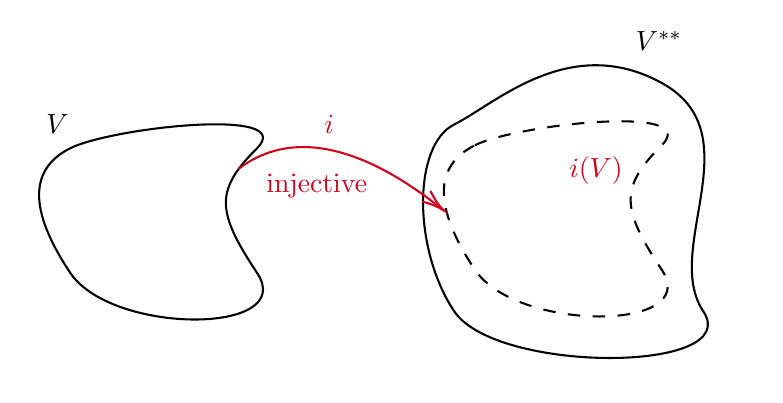
\begin{tikzpicture}[x=0.75pt,y=0.75pt,yscale=-1,xscale=1]
%uncomment if require: \path (0,421); %set diagram left start at 0, and has height of 421

%Shape: Polygon Curved [id:ds23351701075718778] 
\draw   (100,280) .. controls (120,270) and (210,260) .. (190,280) .. controls (170,300) and (170,310) .. (190,340) .. controls (210,370) and (120,370) .. (100,340) .. controls (80,310) and (80,290) .. (100,280) -- cycle ;
%Shape: Polygon Curved [id:ds5106655891262244] 
\draw  [dash pattern={on 4.5pt off 4.5pt}] (295,278.54) .. controls (315,268.54) and (405,258.54) .. (385,278.54) .. controls (365,298.54) and (365,308.54) .. (385,338.54) .. controls (405,368.54) and (315,368.54) .. (295,338.54) .. controls (275,308.54) and (275,288.54) .. (295,278.54) -- cycle ;
%Shape: Polygon Curved [id:ds3732810569342433] 
\draw   (285,268.54) .. controls (305,258.54) and (340.67,224.22) .. (385,248.54) .. controls (429.33,272.87) and (385,328.54) .. (405,358.54) .. controls (425,388.54) and (305,388.54) .. (285,358.54) .. controls (265,328.54) and (265,278.54) .. (285,268.54) -- cycle ;
%Curve Lines [id:da8915674336439121] 
\draw [color={rgb, 255:red, 208; green, 2; blue, 27 }  ,draw opacity=1 ]   (181,290) .. controls (212.85,265.71) and (252.46,287.99) .. (278.81,309.04) ;
\draw [shift={(280,310)}, rotate = 219] [color={rgb, 255:red, 208; green, 2; blue, 27 }  ,draw opacity=1 ][line width=0.75]    (10.93,-3.29) .. controls (6.95,-1.4) and (3.31,-0.3) .. (0,0) .. controls (3.31,0.3) and (6.95,1.4) .. (10.93,3.29)   ;

% Text Node
\draw (87,262.4) node [anchor=north west][inner sep=0.75pt]    {$V$};
% Text Node
\draw (371,222.4) node [anchor=north west][inner sep=0.75pt]    {$V^{**}$};
% Text Node
\draw (221,262.4) node [anchor=north west][inner sep=0.75pt]  [color={rgb, 255:red, 208; green, 2; blue, 27 }  ,opacity=1 ]  {$i$};
% Text Node
\draw (193,291) node [anchor=north west][inner sep=0.75pt]  [color={rgb, 255:red, 208; green, 2; blue, 27 }  ,opacity=1 ] [align=left] {injective};
% Text Node
\draw (339,282.4) node [anchor=north west][inner sep=0.75pt]  [color={rgb, 255:red, 208; green, 2; blue, 27 }  ,opacity=1 ]  {$i( V)$};


\end{tikzpicture}

\end{center}

This canonical embedding is described by `evaluating at $v$'.

\begin{theorem}[Canonical Embedding of $V$ into $V^{**}$]
    There is a natural injective linear map from $V$ to $V^{**}$, called the \vocab{evaluation map}.
\end{theorem}
\begin{proof}
Let $V$ be an $\F$ vector space, and let $v \in V$.
We define the evaluation at $v$ map
$$
\hat{v}: V^* \rightarrow \F \quad \text{by} \quad \hat{v}(\varepsilon) = \varepsilon(v).
$$
Then $\hat{v}(\varepsilon_1 + \lambda \varepsilon_2) = (\varepsilon_1 + \lambda \varepsilon_2)(v) = \varepsilon_1(v) + \lambda \varepsilon_2(v)$, so $\hat{v} \in V^{**}$.

The proof that this is injective is intentionally omitted.
\end{proof}


\begin{theorem}[Canonical Embedding in Finite Dimensions]
    If $V$ is finite dimensional, then the evaluation map is an isomorphism.
\end{theorem}
\begin{proof}
    We know that for $v \in V$ we have the evaluation map $\hat{v} \in V^{**}$. It's easy to see that the map $v \mapsto \hat{v}$ is linear in $v$, so it is left to check that this map is a bijection.

    Let $e \in V \backslash {0}$. We can extend $\{e\}$ to a basis $B = \{e, e_2, \dots, e_n\}$ of $V$. Let $B^*$ be the dual basis of $V$. 
    Then
    $$
    \hat{e}(e^*) = e^*(e) = 1,
    $$
    and in particular, $\hat{e} \neq 0$, so the kernel of the map $v \mapsto \hat{v}$ contains only $0$, and thus it is injective\footnote{This step of the proof has an analogue in infinite dimensions for a certain kind of vector space (Banach space), but requires the use of non-trivial results (the Hahn-Banach theorem).}.

    To see that this map is an isomorphism, we just need to compute dimensions. We know that $\dim V = \dim V^* = \dim (V^*)^* = \dim V^{**}$, and this along with injectivity implies that the map $v \mapsto \hat{v}$ is an isomorphism.
\end{proof}

This canonical embedding allows us to `identify' $V$ and $V^{**}$, which in turn can be used to prove various facts about say the annihilator.

\begin{lemma}[Double Annihilator]
    Let $V$ be a finite dimensional vector space over $\F$, and $U \leq V$. Then
    $\hat{U} = U^{00}$, so after identification of $V$ and $V^{**}$, we have $U = U^{00}$.
\end{lemma}
\begin{proof}
    Let us first show that $U \leq U^{00}$. Indeed, let $u \in U$. Then for all $\varepsilon \in U^0$, $\varepsilon(u) = 0$. But then $\varepsilon(u) = \hat{u}(\varepsilon) = 0$, so $\hat{u} \in U^{00}$, and $\hat{U} \leq U^{00}$.
    
    We can then compute dimensions, and $\dim U^{00} = \dim V - \dim U^{0} = \dim U$, and since $v \mapsto \hat{v}$ is an isomorphism, $\dim \hat{U} = 
    \dim U$. Thus $\dim \hat{U} = \dim U = \dim U^{00}$, and $\hat{U} = U^{00}$.
\end{proof}

\begin{remark}
    With the identification of $V^{**}$ and $V$, for $T \leq V^{*}$ we can define $T^0 = \{v \in V \mid \alpha(v) = 0, \; \forall \alpha \in T\}$.
\end{remark}

These results give us some unsurprising properties which are useful for doing computations.

\begin{lemma}[Sums and Intersections of Annihilators]
    Let $V$ be a finite dimensional vector space over $\F$, and let $U_1, U_2 \leq V$. Then 
    \begin{enumerate}[label=(\roman*)]
        \item $(U_1 + U_2)^0 = U_1^0 \cap U_2^0$;
        \item $(U_1 \cap U_2) = U_1^0 + U_2^0$.
    \end{enumerate}
\end{lemma}
\begin{proof}
    (i) Let $\theta \in V^*$, then $\theta \in (U_1 + U_2)^0$ if and only if $\theta(u_1 + u_2) = 0$ for all $u_1 \in U_1$ and $u_2 \in U_2$. By linearity this is exactly when $\theta(u) = 0$ for $u \in U_1 \cup U_2$, which occurs if and only if $\theta \in U_1^0 \cap U_2^0$.

    (ii) Take the annihilator of the result in (i), and use the fact that $U^{00} = U$.
\end{proof}

\section{Bilinear Forms}

\subsection{Introducing Bilinear Forms}

In the previous section we considered linear maps from a vector space to the scalar field that vector space is over. In this section we will look at a related but interesting set of maps which have \emph{two} arguments and are linear in both.
Such maps are \emph{bilinear forms}.

\begin{definition}[Bilinear Form]
    Let $U$ and $V$ be vector spaces over $\F$. Then $\phi: U \times V \rightarrow \F$ is a \vocab{bilinear form} if it is linear in both components.
\end{definition}

\begin{example}[Examples of Bilinear Forms]
    The following are all bilinear forms.
    \begin{enumerate}[label=(\roman*)]
        \item A canonical example -- the scalar product on $U = V = \R^n$.
        \item The map $V \times V^* \rightarrow \F$ given by $(v, \alpha) \mapsto \alpha(v)$.
        \item For $U = V = \mathcal{C}([0, 1],\R)$ the map
        $
        \phi(f, g) = \int_0^1 f(t) g(t) \dd t.
        $
    \end{enumerate}
\end{example}

There is a standard representation of bilinear forms using matrices.

\begin{definition}[Matrix of a Bilinear Form]
    Let $B = \{u_1, \dots, u_n\}$ be a basis of $U$ and $C = \{v_1, \dots, v_m\}$ be a basis of $V$, and let $\phi: U \times V \rightarrow \F$ be a bilinear form.
    
    We define the \vocab{matrix of $\phi$} with respect to $B$ and $C$ by
    $$
    ([\phi]_{B, C})_{i, j} = \phi(u_i, v_j). 
    $$
\end{definition}

\begin{lemma}[Evaluating a Bilinear Form]
    Let $\phi: U \times V \rightarrow \F$ be a bilinear form, and let $u \in U$ and $v \in V$. Then if $B$ is a basis of $U$ and $C$ is a basis of $V$, we have
    $$
    \phi(u, v) = [u]_B^T [\phi]_{B, C} [v]_C.
    $$
\end{lemma}
\begin{proof}[Proof Sketch]
    Check definitions.
\end{proof}

\begin{remark}
    $[\phi]_{B, C}$ is the unique matrix such that this equation holds.
\end{remark}

It's sometimes useful to study a bilinear form in just one of its arguments. This can be done by considering the induced maps.

\begin{definition}[Induced Map of a Bilinear Form]    
    Let $\phi: U \times V \rightarrow \F$ be a bilinear form. Then $\phi$ determines two linear maps $\phi_L: U \rightarrow V^*$ and $\phi_R: V\rightarrow U^*$, with
    $$
    (\phi_L(u))(v) = \phi(u, v) \quad \text{and} \quad (\phi_R(v))(u) = \phi(u, v).
    $$
\end{definition}

These induced maps are easily obtained from the matrix of the bilinear form.

\begin{lemma}[Matrices of the Induced Maps]
    Let $\phi: U \times V \rightarrow \F$ be a bilinear map.
    Then if $B = \{u_1, \dots, u_n\}$ is a basis of $U$ and $C = \{v_1, \dots, v_m\}$ is a basis of $U$, then if $A = [\phi]_{B, C}$ we have
    $$
    [\phi_R]_{C, B^*} = A \quad \text{and} \quad [\phi_L]_{B, C^*} = A^T.
    $$
\end{lemma}
\begin{proof}[Proof Sketch]
    Check definitions.
\end{proof}

Just as with the linear maps that we studied previously, it's possible look at the kernel of a bilinear map by considering the left and right component.

\begin{definition}[Left/Right Kernel]
    Let $\phi: U \times V \rightarrow \F$ be a bilinear form. Then the \vocab{left kernel} of $\phi$ is $\kernel \phi_L$, and the \vocab{right kernel} of $\phi$ is $\kernel \phi_R$.
\end{definition}

\begin{definition}[Degeneracy]
    We say that a bilinear form $\phi$ is \vocab{non-degenerate} if $\kernel \phi_L = \{0\}$ and $\kernel \phi_R = \{0\}$. Otherwise, we say that $\phi$ is \vocab{degenerate}. 
\end{definition}

\begin{lemma}[Matrix Degeneracy Criterion]
    Let $U$ and $V$ be finite dimensional vector spaces, and 
let $B$ be a basis of $U$ and $C$ be a basis of $V$. 
Suppose $\phi: U \times V \rightarrow \F$ is a bilinear form with matrix $A = [\phi]_{B, C}$. Then $\phi$ is non-degenerate if and only if $A$ is invertible.
\end{lemma}
\begin{proof}
    We know that $\phi$ is non-degenerate if and only if $\kernel \phi_L = \{0\}$ and $\kernel \phi_R = \{0\}$, that is, if and only if $n(A^T) = 0$ and $n(A) = 0$. But then by rank-nullity, we have this if and only if $r(A^T) = \dim U$ and $r(A) = \dim V$, that is, if and only if $A$ is invertible.
\end{proof}

\begin{corollary}
    If $\phi: U \times V \rightarrow \F$ is a non-degenerate bilinear form, then $\dim U = \dim V$.
\end{corollary}

\begin{corollary}[Choosing a Bilinear Form]
    When $U$ and $V$ are finite dimensional vector spaces over $\F$, choosing a non-degenerate bilinear form $\phi: U \times V \rightarrow \F$ is equivalent to choosing an isomorphism $\phi_L : U \rightarrow V^*$.
\end{corollary}

As with matrices for normal linear maps $\alpha: V \rightarrow W$, we can change the basis that the matrix of a bilinear form is represented with.

\begin{proposition}[Change of Basis for Bilinear Forms]
    Let $U$ and $V$ be vector spaces over $\F$ and let $B, B'$ be bases for $U$ and $C, C'$ be bases for $V$. Suppose that $P$ is the change of basis matrix from $B'$ to $B$ and $Q$ is the change of basis matrix from $C'$ to $C$. Then if $\phi: U \times V \rightarrow \F$ is a bilinear form, then
    $$
    [\phi]_{B', C'} = P^T [\phi]_{B, C} Q.
    $$
\end{proposition}
\begin{proof}
    We have
    $$
        \phi(u, v) = [u]^T_B [\phi]_{B, C} [v]_C 
            = (P[u]_{B'})^T [\phi]_{B, C} (Q [v]_{C'}) 
                = [u]^T_{B'} (P^T [\phi]_{B, C} Q) [v]_{C'},
    $$
    and thus $[\phi]_{B', C'} = P^T [\phi]_{B, C} Q$.
\end{proof}

This change of basis formula also allows us to define the rank of a bilinear map and have that definition be well defined.

\begin{definition}[Rank of a Bilinear Map]
    The rank of a bilinear map $\phi$, $r(\phi)$, is the rank of any matrix representation of $\phi$. 
\end{definition}

To see that this is well defined, note that $r(P^T AQ) = r(A)$ for any invertible $P, Q$.

\section{The Trace and Determinant}

We will now look at the determinant and trace, two quantities you may be familiar with from the study of matrices. In this section, we will consider how these can be interpreted in a basis-free way -- that is, how they can be seen as quantities attached to a linear map itself, not just to a particular matrix representation of it.

\subsection{The Trace}

We begin with the trace, which is by far the simpler of the two.

\begin{definition}[Trace]
    Let $A \in \mathcal{M}_{n, n}(\F)$ be a square matrix. We define the trace of $A$ by
    $$
    \tr A = \sum_{i = 1}^n A_{ii}.
    $$
\end{definition}

In particular, we have
$$
\tr \begin{pmatrix}
    a_{11} & \cdots & a_{1n} \\
    \vdots & \ddots & \vdots \\
    a_{n1} & \cdots & a_{nn}
\end{pmatrix} = a_{11} + \cdots + a_{nn}.
$$

\begin{remark}
    The trace is a linear form $\mathcal{M}_{n,n}(\F) \rightarrow \F$ given by $A \mapsto \tr A$.
\end{remark}

The key computational fact about the trace is that it does not notice the order of a product.

\begin{lemma}[Trace of a Product]
    For any matrices $A, B \in \mathcal{M}_{n,n}(\F)$, we have $\tr (AB) = \tr(BA)$.
\end{lemma}
\begin{proof}
    Directly computing, we have
    $$
    \tr (AB) = \sum_{i = 1}^n \sum_{j = 1}^n a_{ij}b_{ji} = \sum_{j = 1}^n \sum_{i = 1}^n b_{ji} a_{ij} = \tr (BA). \qedhere
    $$
\end{proof}

\begin{corollary}[Similar Matrices Have Equal Trace]
    If $A$ and $A'$ are similar matrices, then $\tr A = \tr A'$.
\end{corollary}
\begin{proof}
    If $A' = P^{-1}AP$, then $\tr A' = \tr(P^{-1}(AP)) = \tr((AP)P^{-1}) = \tr A$.
\end{proof}

This corollary is exactly what we need to make a basis-free definition. Recalling that two matrices represent the same endomorphism (in possibly different bases) precisely when they are similar, the following is well defined.

\begin{definition}[Trace of an Endomorphism]
    Let $\alpha: V \rightarrow V$ be an endomorphism of a finite dimensional vector space $V$. The \vocab{trace} of $\alpha$ is $\tr \alpha = \tr [\alpha]_{B, B}$, where $B$ is any basis of $V$.
\end{definition}

As a quick application of thinking this way, the trace interacts with duality in the way you might guess.

\begin{lemma}[Trace of the Dual Map]
    Let $\alpha : V \rightarrow V$ be an endomorphism of a finite dimensional vector space. Then $\tr \alpha^* = \tr \alpha$.
\end{lemma}
\begin{proof}
    Picking a basis $B$ of $V$, we have $\tr \alpha^* = \tr [\alpha^*]_{B^*, B^*} = \tr [\alpha]_{B, B}^T = \tr [\alpha]_{B, B} = \tr \alpha$, since transposing a matrix does not change its diagonal.
\end{proof}

\subsection{Permutations}

The determinant requires a bit more machinery than the trace, and the machinery it requires is that of \emph{permutations}, which we briefly recall from IA Groups.

The \vocab{symmetric group} $S_n$ is the group of permutations of $\{1, \dots, n\}$, that is, the group of bijections $\sigma: \{1, \dots, n\} \rightarrow \{1, \dots, n\}$ under composition. A \vocab{transposition} $(k \; \ell)$ is a permutation which swaps $k$ and $\ell$ and fixes everything else. Every permutation can be written as a product of transpositions, and while such a decomposition is not unique, the \emph{parity} of the number of transpositions used is. This lets us define the \vocab{signature} $\varepsilon: S_n \rightarrow \{\pm 1\}$, with $\varepsilon(\sigma) = 1$ if $\sigma$ is a product of an even number of transpositions and $\varepsilon(\sigma) = -1$ otherwise. Importantly, the signature is a group homomorphism.

\subsection{The Determinant}

With that, we can write down the (somewhat intimidating looking) definition of the determinant.

\begin{definition}[Determinant]
    Let $A \in \mathcal{M}_{n,n}(\F)$. The \vocab{determinant} of $A$ is
    $$
    \det A = \sum_{\sigma \in S_n} \varepsilon(\sigma)\, a_{\sigma(1) 1} a_{\sigma(2) 2} \cdots a_{\sigma(n) n}.
    $$
\end{definition}

Each term in this sum picks exactly one entry from each column of $A$, with no two entries from the same row, and weights the resulting product by a sign. For small $n$, this recovers formulas you already know.

\begin{example}[Determinants of Small Matrices]
    For $n = 2$, the only permutations are the identity and the transposition $(1\;2)$, so
    $$
    \det \begin{pmatrix}
        a_{11} & a_{12} \\ a_{21} & a_{22}
    \end{pmatrix} = a_{11}a_{22} - a_{12}a_{21}.
    $$
    Similarly for $n = 3$, the six permutations of $S_3$ give the familiar six-term formula.
\end{example}

Directly from the definition we can compute the determinant of triangular matrices.

\begin{lemma}[Determinant of a Triangular Matrix]
    If $A$ is an upper (or lower) triangular matrix with diagonal entries $a_{11}, \dots, a_{nn}$, then $\det A = a_{11} a_{22} \cdots a_{nn}$.
\end{lemma}
\begin{proof}
    Suppose $a_{ij} = 0$ for $i > j$. For the term corresponding to $\sigma$ in the sum to be non-zero, we need $\sigma(j) \leq j$ for all $j$. But then $\sigma(1) = 1$, which forces $\sigma(2) = 2$, and so on -- so the only permutation contributing is the identity, and $\det A = a_{11} \cdots a_{nn}$. The lower triangular case is analogous.
\end{proof}

\begin{lemma}[Determinant of the Transpose]
    Let $A \in \mathcal{M}_{n,n}(\F)$. Then $\det A^T = \det A$.
\end{lemma}
\begin{proof}
    Reindexing the product inside the sum using $\sigma^{-1}$, and noting that $\sigma \mapsto \sigma^{-1}$ is a bijection $S_n \rightarrow S_n$ with $\varepsilon(\sigma^{-1}) = \varepsilon(\sigma)$, we get
    \begin{align*}
    \det A &= \sum_{\sigma \in S_n} \varepsilon(\sigma) \prod_{i = 1}^n a_{\sigma(i) i} = \sum_{\sigma \in S_n} \varepsilon(\sigma) \prod_{j = 1}^n a_{j \sigma^{-1}(j)} \\
    &= \sum_{\tau \in S_n} \varepsilon(\tau) \prod_{j = 1}^n a_{j \tau(j)} = \det A^T. \qedhere
    \end{align*}
\end{proof}

\subsection{Volume Forms}

The definition of the determinant above is useful for computing, but it's fair to say it doesn't exactly drip with meaning. The right way to understand the determinant is \emph{geometric}: viewing the columns of $A$ as $n$ vectors in $\F^n$, the determinant is the \emph{signed volume} of the parallelepiped they span.

\begin{center}
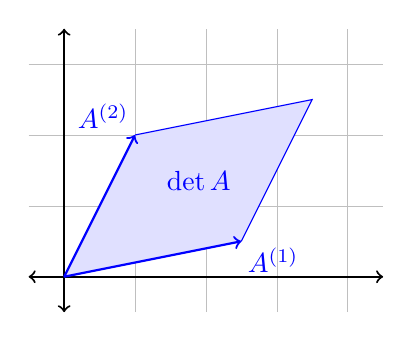
\begin{tikzpicture}[scale=0.9]
    \draw[ultra thin, color=lightgray] (-0.5,-0.5) grid (4.5,3.5);
    \draw[<->] (-0.5,0) -- (4.5,0);
    \draw[<->] (0,-0.5) -- (0,3.5);
    \fill[blue!12] (0,0) -- (2.5,0.5) -- (3.5,2.5) -- (1,2) -- cycle;
    \draw[->, thick, color=blue] (0,0) -- (2.5,0.5) node[below right, inner sep=2pt] {$A^{(1)}$};
    \draw[->, thick, color=blue] (0,0) -- (1,2) node[above left, inner sep=2pt] {$A^{(2)}$};
    \draw[thin, color=blue] (2.5,0.5) -- (3.5,2.5) -- (1,2);
    \node[color=blue] at (1.9,1.35) {$\det A$};
\end{tikzpicture}
\end{center}

To make this precise (and to prove the important properties of the determinant cleanly) we isolate the properties that any sensible notion of `signed volume' should satisfy.

\begin{definition}[Volume Form]
    A \vocab{volume form} $d$ on $\F^n$ is a function $d: \underbrace{\F^n \times \cdots \times \F^n}_{n \text{ times}} \rightarrow \F$ such that:
    \begin{enumerate}[label=(\roman*)]
        \item \emph{$d$ is multilinear}: for each $i$ and each fixed choice of $v_1, \dots, v_{i - 1}, v_{i + 1}, \dots, v_n$, the map $v \mapsto d(v_1, \dots, v_{i-1}, v, v_{i + 1}, \dots, v_n)$ is linear;
        \item \emph{$d$ is alternating}: if $v_i = v_j$ for some $i \neq j$, then $d(v_1, \dots, v_n) = 0$.
    \end{enumerate}
\end{definition}

Both of these are natural if you think of $d$ as measuring volume -- scaling one edge of a parallelepiped scales its volume\footnote{Additivity in each argument is perhaps slightly less obvious, but can be seen with a `shearing' argument.}, and a `parallelepiped' with two equal edges is squashed flat, so should have zero volume.

\begin{lemma}[Determinant is a Volume Form]
    The map $(\F^n)^n \rightarrow \F$ given by $(A^{(1)}, \dots, A^{(n)}) \mapsto \det A$, where $A$ is the matrix with columns $A^{(1)}, \dots, A^{(n)}$, is a volume form.
\end{lemma}
\begin{proof}
    For multilinearity, fix $\sigma \in S_n$ and consider the term $\prod_{i = 1}^n a_{\sigma(i)i}$. This product contains exactly one entry from each column of $A$, so it is linear in each column separately. The determinant is a sum of such terms, so is multilinear.

    For the alternating property, suppose columns $k \neq \ell$ are equal, and let $\tau = (k\;\ell)$. Then $a_{i j} = a_{i \tau(j)}$ for all $i, j$. Splitting $S_n = A_n \cup \tau A_n$ into even permutations and odd permutations, the terms for $\sigma$ and $\tau\sigma$ have equal products but opposite signs, so cancel in pairs. Hence $\det A = 0$.
\end{proof}

\begin{lemma}[Swapping Entries]
    Let $d$ be a volume form. Then swapping two arguments of $d$ changes its sign, that is,
    $$
    d(v_1, \dots, v_i, \dots, v_j, \dots, v_n) = -d(v_1, \dots, v_j, \dots, v_i, \dots, v_n).
    $$
\end{lemma}
\begin{proof}
    Consider $d$ applied with $v_i + v_j$ in \emph{both} the $i$th and $j$th positions. By the alternating property this is zero, and expanding by multilinearity,
    \begin{align*}
    0 &= \underbrace{d(\dots, v_i, \dots, v_i, \dots)}_{= \, 0} + d(\dots, v_i, \dots, v_j, \dots) \\
    &\qquad + d(\dots, v_j, \dots, v_i, \dots) + \underbrace{d(\dots, v_j, \dots, v_j, \dots)}_{=\, 0},
    \end{align*}
    which rearranges to give the result.
\end{proof}

\begin{corollary}[Volume Forms and Permutations]
    If $d$ is a volume form and $\sigma \in S_n$, then $d(v_{\sigma(1)}, \dots, v_{\sigma(n)}) = \varepsilon(\sigma)\, d(v_1, \dots, v_n)$.
\end{corollary}
\begin{proof}
    Write $\sigma$ as a product of transpositions and apply the previous lemma once for each.
\end{proof}

We can now prove the theorem that justifies this whole discussion: up to scaling, the determinant is the \emph{only} volume form on $\F^n$.

\begin{theorem}[Uniqueness of Volume Forms]
    Let $d$ be a volume form on $\F^n$, and let $A$ be a matrix with columns $A^{(1)}, \dots, A^{(n)}$. Then
    $$
    d(A^{(1)}, \dots, A^{(n)}) = \det A \cdot d(e_1, \dots, e_n).
    $$
    In particular, the determinant is the unique volume form with $d(e_1, \dots, e_n) = 1$.
\end{theorem}
\begin{proof}
    Writing $A^{(1)} = \sum_{i = 1}^n a_{i1}e_i$ and using multilinearity in the first argument,
    $$
    d(A^{(1)}, \dots, A^{(n)}) = \sum_{i = 1}^n a_{i1}\, d(e_i, A^{(2)}, \dots, A^{(n)}).
    $$
    Doing the same in every argument, we get
    $$
    d(A^{(1)}, \dots, A^{(n)}) = \sum_{i_1, \dots, i_n} a_{i_1 1} a_{i_2 2}\cdots a_{i_n n}\, d(e_{i_1}, \dots, e_{i_n}).
    $$
    Since $d$ is alternating, the only non-zero terms are those where $i_1, \dots, i_n$ are distinct -- that is, where $i_k = \sigma(k)$ for some permutation $\sigma \in S_n$. Applying the corollary above,
    $$
    d(A^{(1)}, \dots, A^{(n)}) = \sum_{\sigma \in S_n} \varepsilon(\sigma) \prod_{k = 1}^n a_{\sigma(k)k} \cdot d(e_1, \dots, e_n) = \det A \cdot d(e_1, \dots, e_n),
    $$
    as required.
\end{proof}

This uniqueness result is more than just aesthetically pleasing -- it gives essentially free proofs of facts about the determinant that are painful to obtain from the formula. The prime example is multiplicativity.

\begin{theorem}[Determinant is Multiplicative]
    Let $A, B \in \mathcal{M}_{n,n}(\F)$. Then $\det (AB) = \det A \det B$.
\end{theorem}
\begin{proof}
    Fixing $A$, define $d_A: (\F^n)^n \rightarrow \F$ by
    $$
    d_A(v_1, \dots, v_n) = \det(Av_1, \dots, Av_n),
    $$
    where the right hand side denotes the determinant of the matrix with the given columns. Since $v \mapsto Av$ is linear and $\det$ is multilinear, $d_A$ is multilinear, and if $v_i = v_j$ then $Av_i = Av_j$, so $d_A$ is alternating. Thus $d_A$ is a volume form, and by uniqueness $d_A = C_A \det$ for the constant
    $$
    C_A = d_A(e_1, \dots, e_n) = \det(Ae_1, \dots, Ae_n) = \det A,
    $$
    since $Ae_i$ is exactly the $i$th column of $A$. Applying this with the columns of $B$,
    $$
    \det(AB) = d_A(B^{(1)}, \dots, B^{(n)}) = \det A \det B. \qedhere
    $$
\end{proof}

\subsection{Singular and Non-Singular Matrices}

The determinant gives us a clean test for invertibility.

\begin{definition}[Singular Matrices]
    A square matrix $A$ is \vocab{singular} if $\det A = 0$, and \vocab{non-singular} otherwise.
\end{definition}

\begin{theorem}[Determinant Criterion for Invertibility]
    Let $A \in \mathcal{M}_{n,n}(\F)$. Then the following are equivalent:
    \begin{enumerate}[label=(\roman*)]
        \item $A$ is invertible,
        \item $A$ is non-singular,
        \item $r(A) = n$.
    \end{enumerate}
\end{theorem}
\begin{proof}
    \emph{(i) implies (ii)}. If $A$ is invertible then $\det A \det A^{-1} = \det (AA^{-1}) = \det I = 1$, so $\det A \neq 0$.

    \emph{(i) is equivalent to (iii)}. This is the rank-nullity theorem: $A$ is invertible if and only if the linear map it represents is bijective, which happens if and only if it is surjective, that is $r(A) = n$.

    \emph{(ii) implies (iii)}. We show the contrapositive. If $r(A) < n$, then the columns $A^{(1)}, \dots, A^{(n)}$ are linearly dependent, so some $A^{(j)} = -\frac{1}{\lambda_j}\sum_{i \neq j} \lambda_i A^{(i)}$ for scalars $\lambda_i$ with $\lambda_j \neq 0$. Expanding $\det A$ using multilinearity in the $j$th column expresses it as a sum of determinants of matrices with two equal columns, all of which vanish. So $\det A = 0$.
\end{proof}

\subsection{The Determinant of a Linear Map}

We can now play the same game that we played with the trace.

\begin{lemma}[Similar Matrices Have Equal Determinant]
    If $A' = P^{-1} A P$, then $\det A' = \det A$.
\end{lemma}
\begin{proof}
    Using multiplicativity and $\det P^{-1}\det P = 1$, we have
    $$
    \det (P^{-1}AP) = \det P^{-1} \det A \det P = \det A. \qedhere
    $$
\end{proof}

\begin{definition}[Determinant of an Endomorphism]
    Let $\alpha: V \rightarrow V$ be an endomorphism of a finite dimensional vector space $V$. The \vocab{determinant} of $\alpha$ is $\det \alpha = \det [\alpha]_{B, B}$, where $B$ is any basis of $V$.
\end{definition}

The properties of the matrix determinant transfer directly: $\det (\operatorname{id}) = 1$, $\det (\alpha\beta) = \det \alpha \det \beta$, and $\alpha$ is invertible if and only if $\det \alpha \neq 0$, in which case $\det \alpha^{-1} = (\det \alpha)^{-1}$.

There is one more computational result that will be repeatedly useful when we study eigenvalues.

\begin{lemma}[Determinant of Block Triangular Matrices]
    Let $A \in \mathcal{M}_{k,k}(\F)$, $B \in \mathcal{M}_{\ell,\ell}(\F)$ and $C \in \mathcal{M}_{k, \ell}(\F)$, and consider the block matrix
    $$
    M = \left(\begin{array}{ c | c }
        A & C \\
        \hline
        0 & B
      \end{array}\right).
    $$
    Then $\det M = \det A \det B$.
\end{lemma}
\begin{proof}
    Let $n = k + \ell$ and write $M = (m_{ij})$. In the sum
    $$
    \det M = \sum_{\sigma \in S_n} \varepsilon(\sigma) \prod_{i = 1}^n m_{\sigma(i)i},
    $$
    the term for $\sigma$ vanishes unless $\sigma(i) \leq k$ for all $i \leq k$ (as the bottom-left block is zero). Such $\sigma$ decompose uniquely as $\sigma = \sigma_1\sigma_2$ where $\sigma_1$ permutes $\{1, \dots, k\}$ and $\sigma_2$ permutes $\{k + 1, \dots, n\}$, with $\varepsilon(\sigma) = \varepsilon(\sigma_1)\varepsilon(\sigma_2)$. The sum then factors as
    $$
    \det M = \left(\sum_{\sigma_1} \varepsilon(\sigma_1) \prod_{i = 1}^{k} m_{\sigma_1(i)i}\right)\left(\sum_{\sigma_2} \varepsilon(\sigma_2) \prod_{i = k+1}^{n} m_{\sigma_2(i)i}\right) = \det A \det B. \qedhere
    $$
\end{proof}

Applying this repeatedly, a block \emph{upper} triangular matrix has determinant equal to the product of the determinants of its diagonal blocks.

\subsection{Expanding Determinants and the Adjugate}

The formula defining the determinant has $n!$ terms, so is rarely how you want to compute one. A more practical approach reduces an $n \times n$ determinant to a combination of $(n-1) \times (n-1)$ determinants.

\begin{definition}[Minor]
    Let $A \in \mathcal{M}_{n,n}(\F)$ and $i, j \in \{1, \dots, n\}$. The \vocab{minor} $A_{\widehat{i}\widehat{j}} \in \mathcal{M}_{n - 1, n-1}(\F)$ is the matrix obtained from $A$ by deleting the $i$th row and $j$th column.
\end{definition}

\begin{lemma}[Row and Column Expansions]
    Let $A \in \mathcal{M}_{n,n}(\F)$. Then for any fixed column $j$,
    $$
    \det A = \sum_{i = 1}^n (-1)^{i + j} a_{ij} \det A_{\widehat{i}\widehat{j}},
    $$
    and for any fixed row $i$, we similarly have $\det A = \sum_{j = 1}^n (-1)^{i+j}a_{ij} \det A_{\widehat{i}\widehat{j}}$.
\end{lemma}
\begin{proof}
    Write the $j$th column as $A^{(j)} = \sum_{i = 1}^n a_{ij}e_i$. By multilinearity,
    $$
    \det A = \sum_{i = 1}^n a_{ij} \det (A^{(1)}, \dots, e_i, \dots, A^{(n)}),
    $$
    with $e_i$ in the $j$th position. Now move the $j$th column to the front ($j - 1$ adjacent swaps) and the $i$th row to the top ($i - 1$ adjacent swaps), picking up the sign $(-1)^{i + j - 2} = (-1)^{i+j}$. The resulting matrix is block triangular with top-left block $(1)$ and bottom-right block $A_{\widehat{i}\widehat{j}}$, so by the block triangular lemma,
    $$
    \det(A^{(1)}, \dots, e_i, \dots, A^{(n)}) = (-1)^{i + j}\det A_{\widehat{i}\widehat{j}},
    $$
    giving the column expansion. The row expansion follows by transposing.
\end{proof}

Collecting these signed minors into a matrix gives us an explicit (if computationally expensive) formula for the inverse of a matrix.

\begin{definition}[Adjugate]
    Let $A \in \mathcal{M}_{n,n}(\F)$. The \vocab{adjugate} of $A$ is the $n \times n$ matrix $\adj A$ with
    $$
    (\adj A)_{ij} = (-1)^{i + j} \det A_{\widehat{j}\widehat{i}}.
    $$
\end{definition}

Note the transposition of indices -- the $(i,j)$ entry of the adjugate involves deleting row $j$ and column $i$. In the notation of the proof above, $(\adj A)_{ji} = \det(A^{(1)}, \dots, e_i, \dots, A^{(n)})$ with $e_i$ in position $j$.

\begin{theorem}[Adjugate Formula]
    Let $A \in \mathcal{M}_{n,n}(\F)$. Then
    $$
    (\adj A) A = (\det A) I.
    $$
    In particular, if $A$ is invertible then
    $$
    A^{-1} = \frac{1}{\det A} \adj A.
    $$
\end{theorem}
\begin{proof}
    On the diagonal, the $(j, j)$ entry of $(\adj A)A$ is
    $$
    \sum_{i = 1}^n (\adj A)_{ji} a_{ij} = \sum_{i = 1}^n (-1)^{i + j} a_{ij}\det A_{\widehat{i}\widehat{j}} = \det A,
    $$
    by the column expansion. Off the diagonal, for $j \neq k$ the $(j, k)$ entry is
    $$
    \sum_{i = 1}^n (\adj A)_{ji} a_{ik} = \sum_{i = 1}^n a_{ik} \det (A^{(1)}, \dots, \underbrace{e_i}_{j\text{th}}, \dots, A^{(n)}) = \det(A^{(1)}, \dots, \underbrace{A^{(k)}}_{j\text{th}}, \dots, A^{(n)})
    $$
    after reassembling using multilinearity. But this last determinant has the column $A^{(k)}$ appearing twice (in positions $j$ and $k$), so vanishes.
\end{proof}

\subsection{Cramer's Rule}

Finally, the adjugate machinery gives us an algorithm for computing the unique solution to $Ax = b$ without computing $A^{-1}$.

\begin{proposition}[Cramer's Rule]
    Let $A \in \mathcal{M}_{n , n}(\F)$ be an invertible matrix, and let $b \in \F^n$. Then the unique solution to $Ax = b$ is given by
    $$
    x_i = \frac{1}{\det A} \det(A_{\widehat{i}b}),
    $$
    where $A_{\widehat{i}b}$ is the matrix obtained by replacing the $i$th column of $A$ by $b$.
\end{proposition}
\begin{proof}
    Since $A$ is invertible, there exists a unique $x \in \F^n$ with $Ax = b$. Then
    computing we have
    \begin{align*}
        \det(A_{\widehat{i}b}) &= \det(A^{(1)}, \dots, A^{(i - 1)}, b, A^{(i + 1)}, \dots, A^{(n)}) \\
        &= \det(A^{(1)}, \dots, A^{(i - 1)}, Ax, A^{(i + 1)}, \dots, A^{(n)}) \\
        &= \det\left(A^{(1)}, \dots, A^{(i - 1)}, \sum_{j = 1}^n x_j A^{(j)}, A^{(i + 1)}, \dots, A^{(n)}\right) \\
        &= x_i \det(A^{(1)}, \dots, A^{(i - 1)}, A^{(i)}, A^{(i + 1)}, \dots, A^{(n)})  \\
        &= x_i \det A,
    \end{align*}
    where in the second-to-last step every other term vanishes since it is the determinant of a matrix with a repeated column.
\end{proof}

\section{Diagonalization, Eigenvectors and Eigenvalues}


\subsection{Diagonal and Triangular Matrices}

We are now going to take the first steps towards the diagonalisation of endomorphisms. 
Given a finite dimensional vector space $V$ over $\F$ and some endomorphism $\alpha: V \rightarrow V$, we are going to be guided by the following general problem:
\begin{center}\color{blue}
    Can we find a basis $B$ of $V$ such that in this basis $[\alpha]_{B, B}$ has a `nice' form?
\end{center}
With this in mind, we will first care about when this `nice' form is a diagonal matrix, or more generally a triangular matrix.


\begin{definition}[Diagonalizable]
    Let $V$ be a vector space and let $\alpha: V \rightarrow V$ be a linear map. We say that $\alpha$ is \vocab{diagonalizable} if there is a basis $B$ of $V$ such that
    $$
    [\alpha]_{B, B} = \begin{pmatrix}
        \lambda_1 & \cdots & 0 \\
        \vdots & \ddots & \vdots \\
        0 & \cdots & \lambda_n
    \end{pmatrix}
    $$
    where $\lambda_i \in \F$.
\end{definition}

\begin{definition}[Triangulable]    
    Let $V$ be a vector space and let $\alpha: V \rightarrow V$ be a linear map. We say that $\alpha$ is \vocab{triangulable} if there is a basis $B$ of $V$ such that
    $$
    [\alpha]_{B, B} = \begin{pmatrix}
        \lambda_1 & \cdots & * \\
        \vdots & \ddots & \vdots \\
        0 & \cdots & \lambda_n
    \end{pmatrix}
    $$
    where $\lambda_i \in \F$. 
\end{definition}


We will see that when thinking about such matrices, we will frequently turn to the concept of eigenvectors and eigenvalues.

\begin{definition}[Eigenvectors and Eigenvalues]
    If $V $ is a vector space over $\F$ and $\alpha: V \rightarrow V$ is a linear map, we say that $\lambda \in \F$ is a \vocab{eigenvalue} if there exists some $v \in V \backslash\{0\}$ such that $\alpha(v) = \lambda v$. We say that $v$ is a corresponding \vocab{eigenvector}.
\end{definition}

\begin{definition}[Eigenspace]
    If $\lambda$ is an eigenvalue of a linear map $\alpha: V \rightarrow V$, we define the corresponding \vocab{eigenspace} to be the subspace $V_\lambda = \{v \in V \mid \alpha(v) = \lambda v\}$.
\end{definition}

When computing eigenvalues we frequently employ the following lemma.

\begin{lemma}[Computing Eigenvalues]
    Let $V$ be a vector space over $\F$, and
    let $\alpha: V \rightarrow V$ be a linear map. Then $\lambda \in \F$ is an eigenvalue if and only if $\det(\alpha - \lambda \operatorname{id}) = 0$.
\end{lemma}
\begin{proof}
    There exists $v \in V \backslash\{0\}$ with $\alpha(v) = \lambda v$ if and only if $\kernel (\alpha - \lambda \operatorname{id}) \neq \{0\}$. This occurs if and only if $\alpha - \lambda \operatorname{id}$ is not injective, and since $\alpha$ is an endomorphism, this occurs if and only if $\alpha - \lambda \operatorname{id}$ is not invertible, that is, if $\det(\alpha - \lambda \operatorname{id}) = 0$.
\end{proof}

Applying this lemma gives us a polynomial in $\lambda$ which one must find the roots of to obtain the eigenvalues of the linear map. We call this polynomial the \emph{characteristic polynomial}.

\begin{definition}[Characteristic Polynomial]
    Let $\alpha: V \rightarrow V$ be an endomorphism. Then the \vocab{characteristic polynomial}\footnote{It should be checked that this definition is basis free, but this is straightforward.} of $\alpha$ is $\chi_{\alpha}(\lambda) = \det(\alpha - \lambda \operatorname{id})$.
\end{definition}

The heart of the matter is the following criterion of triangulability.

\begin{theorem}[Triangulability Criterion]
    Let $V$ be a vector space over $\F$.
    A linear map $\alpha: V \rightarrow V$ is triangulable if and only if
    $$
    \chi_{\alpha}(t) = c \prod_{i = 1}^n (t - \lambda_i),
    $$
    for some $c, \lambda_i\in \F$.
\end{theorem}
\begin{proof}
    Suppose $\alpha$ was triangulable. Then for some basis $B$ of $V$ we have
    $$
    [\alpha]_{B, B} = \begin{pmatrix}
        \lambda_1 & \cdots & * \\
        \vdots & \ddots & \vdots \\
        0 & \cdots & \lambda_n
    \end{pmatrix}, 
    $$
    and so
    $$
    \chi_{\alpha}(t) = \det  \begin{pmatrix}
        \lambda_1 - t & \cdots & * \\
        \vdots & \ddots & \vdots \\
        0 & \cdots & \lambda_n - t
    \end{pmatrix} = \prod_{i = 1}^n(\lambda_i - t),
    $$
    which is of the required form.

    Now suppose that this criterion holds. We will prove by induction on $n = \dim V$ that it implies triangulability. For $n = 1$, we are immediately done, so suppose that $n > 1$. Then let $\lambda$ be a root of $\chi_{\alpha}(t)$ (which exists by assumption). Then $\lambda$ is an eigenvalue of $\alpha$. Let $U = V_\lambda$ be the corresponding eigenspace, and let $\{v_1, \dots, v_k\}$ be a basis of $U$. We can complete this to a basis $B = \{v_1, \dots, v_n\}$ of $V$. So then
    $$
    [\alpha]_{B, B} = \left(\begin{array}{ c | c }
                \lambda I & *\\
                \hline
                0 & C
              \end{array}\right).
    $$
    Now $\alpha$ induces an endomorphism $\overline{\alpha} : V / U \rightarrow V / U$, and $C$ is the matrix of $\overline{\alpha}$ with respect to the basis $\{v_{k + 1} + U, \dots, v_n + U\}$. The characteristic polynomial of $\overline{\alpha}$ divides that of $\alpha$, so it too is a product of linear factors, and by induction we can write $\overline{\alpha}$ in triangular form by choosing an appropriate basis $\{v_{k + 1}' + U, \dots, v_n' + U\}$ of $V/U$. Taking the basis $B' = \{v_1, \dots, v_k, v_{k + 1}', \dots, v_n'\}$ then gives us $[\alpha]_{B', B'}$ in triangular form.
\end{proof}
\begin{remark}
    By the fundamental theorem of algebra, if $\F = \C$, then every matrix is triangulable.
\end{remark}

\subsection{Polynomials}

Before we can get a criterion for \emph{diagonalisability}, we need to set up a small dictionary between endomorphisms and polynomials. Let's first recall some basic facts about polynomials over a field $\F$. We write $\F[t]$ for the vector space of polynomials
$$
f(t) = a_n t^n + a_{n - 1}t^{n - 1} + \cdots + a_1 t + a_0
$$
with coefficients in $\F$, and $\deg f$ for the degree of $f$. The facts we will need are the following.
\begin{enumerate}[label=(\roman*)]
    \item If $\lambda$ is a root of $f$, then $(t - \lambda)$ divides $f$. This can be seen by writing $f(t) = f(t) - f(\lambda)$ and factoring $(t - \lambda)$ out of each $t^k - \lambda^k$.
    \item We say $\lambda$ is a root of \vocab{multiplicity} $k$ if $(t - \lambda)^k$ divides $f$ but $(t - \lambda)^{k + 1}$ does not. A non-zero polynomial of degree $n$ has at most $n$ roots counted with multiplicity.
    \item Two polynomials of degree less than $n$ agreeing at $n$ distinct points are equal (their difference has too many roots).
    \item \emph{The fundamental theorem of algebra}: every non-constant $f \in \C[t]$ has a complex root, and hence factors completely into linear factors.
    \item Given polynomials $a, b \in \F[t]$ with $b \neq 0$, there are polynomials $q, r$ with $a = qb + r$ and $\deg r < \deg b$ (polynomial division).
\end{enumerate}

The dictionary is then this: given a polynomial $p(t) = a_n t^n + \cdots + a_0$ and an endomorphism $\alpha$ of $V$, we can form the endomorphism
$$
p(\alpha) = a_n \alpha^n + a_{n-1}\alpha^{n - 1} + \cdots + a_1 \alpha + a_0 \operatorname{id},
$$
where $\alpha^k$ denotes $k$-fold composition. Similarly for a square matrix $A$ we define $p(A) = a_n A^n + \cdots + a_1 A + a_0 I$. Note that any two polynomials in the same $\alpha$ commute with each other -- this simple observation gets used constantly below.

\subsection{A Criterion for Diagonalisability}

We saw above that triangulability is governed by the characteristic polynomial. Diagonalisability turns out to be governed by polynomials too, in a rather clean way.

\begin{theorem}[Diagonalisability Criterion]
    Let $V$ be a finite dimensional vector space over $\F$, and let $\alpha: V \rightarrow V$ be an endomorphism. Then $\alpha$ is diagonalisable if and only if there is a non-zero polynomial $p$ that is a product of \emph{distinct} linear factors such that $p(\alpha) = 0$.
\end{theorem}
\begin{proof}
    Suppose first that $\alpha$ is diagonalisable, with distinct eigenvalues $\lambda_1, \dots, \lambda_k$, and set $p(t) = \prod_{i = 1}^k (t - \lambda_i)$. If $v$ is a basis vector in the diagonalising basis, then $\alpha(v) = \lambda_i v$ for some $i$, and since the factors of $p(\alpha)$ commute we can apply $(\alpha - \lambda_i \operatorname{id})$ to $v$ first, giving $p(\alpha)(v) = 0$. Since $p(\alpha)$ kills a basis, $p(\alpha) = 0$.

    The converse is the interesting direction. Suppose $p(\alpha) = 0$ where $p(t) = \prod_{i = 1}^k (t - \lambda_i)$ with $\lambda_1, \dots, \lambda_k$ distinct, and let $V_{\lambda_i} = \kernel (\alpha - \lambda_i \operatorname{id})$. We claim that
    $$
    V = \bigoplus_{i = 1}^k V_{\lambda_i},
    $$
    which suffices, since choosing a basis of each eigenspace and taking their union then gives a basis of $V$ consisting of eigenvectors.

    To prove the claim, consider the \emph{Lagrange interpolation} polynomials
    $$
    q_j(t) = \prod_{i \neq j} \frac{t - \lambda_i}{\lambda_j - \lambda_i},
    $$
    which are engineered so that $q_j(\lambda_i) = \delta_{ij}$. The sum $q = q_1 + \cdots + q_k$ has degree at most $k - 1$ and takes the value $1$ at the $k$ distinct points $\lambda_1, \dots, \lambda_k$, so $q \equiv 1$.

    Now define $\pi_j = q_j(\alpha)$. By the above, $\sum_{j = 1}^k \pi_j = \operatorname{id}$, so every $v \in V$ decomposes as
    $$
    v = \sum_{j = 1}^k \pi_j (v).
    $$
    Moreover each $\pi_j(v)$ lands in the eigenspace $V_{\lambda_j}$: up to a scalar, $(\alpha - \lambda_j \operatorname{id}) \circ q_j(\alpha)$ is exactly $p(\alpha) = 0$, so $(\alpha - \lambda_j \operatorname{id})\pi_j(v) = 0$. Hence $V = \sum_{j} V_{\lambda_j}$.

    It remains to check the sum is direct. Note that if $v \in V_{\lambda_j}$, then applying $q_j(\alpha)$ replaces each factor $(\alpha - \lambda_i\operatorname{id})$ acting on $v$ by the scalar $(\lambda_j - \lambda_i)$, so $\pi_j(v) = q_j(\lambda_j) v = v$; and if $v \in V_{\lambda_i}$ with $i \neq j$ then some factor of $q_j(\alpha)$ kills $v$, so $\pi_j(v) = 0$. So suppose
    $$
    v_1 + v_2 + \cdots + v_k = 0, \quad v_i \in V_{\lambda_i}.
    $$
    Applying $\pi_j$ to both sides kills every term except the $j$th, leaving $v_j = 0$. This holds for each $j$, so the decomposition of $0$ is unique and the sum is direct.
\end{proof}

\begin{remark}
    Along the way we proved something useful in its own right: for \emph{any} endomorphism $\alpha$, the sum of eigenspaces corresponding to distinct eigenvalues is always direct. Diagonalisability fails only when this direct sum is a proper subspace of $V$.
\end{remark}

This criterion can feel abstract, so let's see it do something impressive with almost no work.

\begin{example}[Matrices of Finite Order]
    Let $A \in \mathcal{M}_{n,n}(\C)$ with $A^m = I$ for some $m \geq 1$. Then $A$ is diagonalisable, since the polynomial
    $$
    p(t) = t^m - 1 = \prod_{j = 1}^{m} (t - e^{2\pi i j / m})
    $$
    is a product of distinct linear factors and satisfies $p(A) = 0$.
\end{example}

As another application, we can answer the natural question of when two diagonalisable maps can be diagonalised \emph{at the same time}.

\begin{theorem}[Simultaneous Diagonalisation]
    Let $\alpha, \beta$ be diagonalisable endomorphisms of a finite dimensional vector space $V$. Then $\alpha$ and $\beta$ are \vocab{simultaneously diagonalisable} (there is a single basis $B$ with both $[\alpha]_{B,B}$ and $[\beta]_{B,B}$ diagonal) if and only if $\alpha\beta = \beta\alpha$.
\end{theorem}
\begin{proof}
    One direction is immediate: diagonal matrices commute, so if $[\alpha]_{B,B}$ and $[\beta]_{B,B}$ are both diagonal then $\alpha\beta = \beta\alpha$.

    Conversely, suppose $\alpha$ and $\beta$ commute. Since $\alpha$ is diagonalisable, $V = \bigoplus_{i = 1}^k V_{\lambda_i}$ where $\lambda_1, \dots, \lambda_k$ are its distinct eigenvalues. The key point is that $\beta$ preserves each eigenspace of $\alpha$: for $v \in V_{\lambda_j}$,
    $$
    \alpha(\beta(v)) = \beta(\alpha(v)) = \beta(\lambda_j v) = \lambda_j \beta(v),
    $$
    so $\beta(v) \in V_{\lambda_j}$. Now $\beta$ is diagonalisable, so some polynomial $p$ with distinct linear factors has $p(\beta) = 0$, and hence certainly $p(\beta|_{V_{\lambda_j}}) = 0$. So each restriction $\beta|_{V_{\lambda_j}}$ is diagonalisable by our criterion, and we may pick a basis $B_j$ of $V_{\lambda_j}$ consisting of eigenvectors of $\beta$. Since each $B_j$ consists of $\lambda_j$-eigenvectors of $\alpha$ as well, the union $B = B_1 \cup \cdots \cup B_k$ diagonalises both maps simultaneously.
\end{proof}

\subsection{The Minimal Polynomial}

The diagonalisability criterion asks whether \emph{some} polynomial with distinct linear factors kills $\alpha$. It is natural to focus on the smallest polynomial killing $\alpha$.

\begin{definition}[Minimal Polynomial]
    Let $\alpha$ be an endomorphism of a finite dimensional vector space $V$. The \vocab{minimal polynomial} $m_\alpha$ of $\alpha$ is the non-zero monic polynomial of least degree such that $m_\alpha(\alpha) = 0$.
\end{definition}

Some polynomial killing $\alpha$ certainly exists: $\dim \mathcal{L}(V, V) = n^2$, so the $n^2 + 1$ endomorphisms $\operatorname{id}, \alpha, \alpha^2, \dots, \alpha^{n^2}$ are linearly dependent, and any dependence gives a polynomial vanishing at $\alpha$.

\begin{lemma}[Divisibility Property of the Minimal Polynomial]
    Let $\alpha$ be an endomorphism of $V$ and $p \in \F[t]$. Then $p(\alpha) = 0$ if and only if $m_\alpha$ divides $p$. In particular, the minimal polynomial is unique.
\end{lemma}
\begin{proof}
    If $m_\alpha$ divides $p$, say $p = m_\alpha q$, then $p(\alpha) = m_\alpha(\alpha)q(\alpha) = 0$. Conversely, suppose $p(\alpha) = 0$, and divide with remainder: $p = q m_\alpha + r$ with $\deg r < \deg m_\alpha$. Evaluating at $\alpha$ gives $r(\alpha) = 0$, and by minimality of $\deg m_\alpha$ this forces $r \equiv 0$, so $m_\alpha$ divides $p$.

    For uniqueness, two monic minimal polynomials must divide each other and have the same degree, so are equal.
\end{proof}

With this language, our diagonalisability criterion can be restated: \emph{$\alpha$ is diagonalisable if and only if $m_\alpha$ is a product of distinct linear factors}. (If some product of distinct linear factors kills $\alpha$, then $m_\alpha$ divides it, so $m_\alpha$ is itself such a product.)

\begin{example}[Telling Matrices Apart]
    Consider the matrices
    $$
    A = \begin{pmatrix} 1 & 0 \\ 0 & 1\end{pmatrix} \quad \text{and} \quad B = \begin{pmatrix} 1 & 1 \\ 0 & 1\end{pmatrix}.
    $$
    Both satisfy $p(t) = (t - 1)^2$, i.e. $p(A) = p(B) = 0$, so both minimal polynomials divide $(t-1)^2$. For $A$ we have $A - I = 0$, so $m_A(t) = t - 1$; but $B - I \neq 0$, so $m_B(t) = (t - 1)^2$. In particular $B$ is \emph{not} diagonalisable, since its minimal polynomial has a repeated root.
\end{example}

\subsection{The Cayley-Hamilton Theorem}

We now come to one of the most famous theorems of linear algebra, relating the two polynomials we have attached to an endomorphism: \emph{every endomorphism satisfies its own characteristic polynomial}.

\begin{theorem}[Cayley-Hamilton]
    Let $\alpha$ be an endomorphism of a finite dimensional vector space $V$. Then $\chi_\alpha(\alpha) = 0$. Equivalently, $m_\alpha$ divides $\chi_\alpha$.
\end{theorem}

Before the proof, one warning: it is tempting to argue `$\chi_\alpha(t) = \det (\alpha - t\operatorname{id})$, so $\chi_\alpha(\alpha) = \det(\alpha - \alpha) = 0$'. This is nonsense -- $\chi_\alpha(\alpha)$ is an \emph{endomorphism}, not a scalar, and substituting a matrix into the determinant formula in this way is not a valid operation.

We will give two proofs: a clean geometric one for $\F = \C$ (which also covers $\F = \R$, viewing a real matrix as a complex one), and an algebraic one that works over any field.

\begin{proof}[Proof (over $\C$)]
    Since $\F = \C$, we can pick a basis $B = \{v_1, \dots, v_n\}$ in which $A = [\alpha]_{B,B}$ is upper triangular with diagonal entries $a_1, \dots, a_n$, so that
    $$
    \chi_\alpha(t) = \prod_{i = 1}^n (a_i - t).
    $$
    Let $U_j = \langle v_1, \dots, v_j\rangle$, so that $U_0 = \{0\} \leq U_1 \leq \cdots \leq U_n = V$. Triangularity says exactly that $\alpha(U_j) \leq U_j$, and moreover $(\alpha - a_j \operatorname{id})(U_j) \leq U_{j - 1}$, since the $j$th column of $A - a_j I$ has zero entries from row $j$ downwards.

    Now take any $v \in V = U_n$ and feed it through the factors of $\chi_\alpha(\alpha)$ from the right:
    $$
    \chi_\alpha(\alpha)(v) = (\alpha - a_1 \operatorname{id}) \cdots (\alpha - a_{n-1}\operatorname{id}) \underbrace{(\alpha - a_n \operatorname{id})(v)}_{\in\, U_{n - 1}}.
    $$
    Each successive factor pushes the vector down one step in the chain of subspaces, so after all $n$ factors we land in $U_0 = \{0\}$. Hence $\chi_\alpha(\alpha) = 0$.
\end{proof}

\begin{proof}[Proof (any field)]
    Let $A$ be the matrix of $\alpha$ in some basis, and write
    $$
    \det(tI - A) = (-1)^n \chi_A(t) = t^n + a_{n -1}t^{n-1} + \cdots + a_1 t + a_0.
    $$
    Recall the adjugate formula $(\adj B) B = (\det B) I$, and apply it with $B = tI - A$. Every entry of $\adj(tI - A)$ is (up to sign) the determinant of an $(n-1) \times (n-1)$ submatrix of $tI - A$, hence a polynomial in $t$ of degree at most $n - 1$. Collecting coefficients, we can write
    $$
    \adj(tI - A) = B_{n-1}t^{n-1} + \cdots + B_1 t + B_0
    $$
    for some matrices $B_i \in \mathcal{M}_{n,n}(\F)$. The adjugate formula then reads
    $$
    (B_{n-1}t^{n - 1} + \cdots + B_0)(tI - A) = (t^n + a_{n-1}t^{n-1} + \cdots + a_0) I,
    $$
    and since this holds for all $t$ (as an identity of polynomials with matrix coefficients), we may equate the coefficients of each power of $t$:
    \begin{align*}
        t^n &: \quad B_{n - 1} = I \\
        t^{n-1} &: \quad B_{n-2} - B_{n-1}A = a_{n-1}I\\
        &\;\; \vdots\\
        t^1 &: \quad B_0 - B_1 A = a_1 I \\
        t^0 &: \quad -B_0 A = a_0 I.
    \end{align*}
    Multiplying the $t^k$ relation on the right by $A^k$ and summing all of the relations, the left hand side telescopes to zero, leaving
    $$
    0 = A^n + a_{n-1}A^{n-1} + \cdots + a_1 A + a_0 I = (-1)^n\chi_A(A),
    $$
    as required.
\end{proof}

\subsection{Multiplicities of Eigenvalues}

We now have three numbers we can attach to each eigenvalue of an endomorphism, and comparing them will give us a rather complete picture of diagonalisability.

\begin{definition}[Algebraic and Geometric Multiplicity]
    Let $\lambda$ be an eigenvalue of an endomorphism $\alpha$ of $V$. We define:
    \begin{enumerate}[label=(\roman*)]
        \item the \vocab{algebraic multiplicity} $a_\lambda$, the multiplicity of $\lambda$ as a root of $\chi_\alpha$,
        \item the \vocab{geometric multiplicity} $g_\lambda = \dim V_\lambda$, the dimension of the corresponding eigenspace,
        \item the multiplicity $c_\lambda$ of $\lambda$ as a root of the minimal polynomial $m_\alpha$.
    \end{enumerate}
\end{definition}

\begin{lemma}[Comparing Multiplicities]
    If $\lambda$ is an eigenvalue of $\alpha$, then
    $$
    1 \leq g_\lambda \leq a_\lambda \quad \text{and} \quad 1 \leq c_\lambda \leq a_\lambda.
    $$
\end{lemma}
\begin{proof}
    Since $\lambda$ is an eigenvalue there is a non-zero eigenvector, so $g_\lambda \geq 1$. For $g_\lambda \leq a_\lambda$, pick a basis $\{v_1, \dots, v_{g_\lambda}\}$ of $V_\lambda$ and extend to a basis $B$ of $V$. Then
    $$
    [\alpha]_{B, B} = \left(\begin{array}{ c | c }
        \lambda I_{g_\lambda} & * \\
        \hline
        0 & A_1
      \end{array}\right),
    $$
    and expanding using the block triangular lemma, $\chi_\alpha(t) = (\lambda - t)^{g_\lambda}\det(A_1 - tI)$. So $(t - \lambda)^{g_\lambda}$ divides $\chi_\alpha(t)$, that is, $g_\lambda \leq a_\lambda$.

    For $c_\lambda$: by Cayley-Hamilton, $m_\alpha$ divides $\chi_\alpha$, so $c_\lambda \leq a_\lambda$. And if $v$ is a $\lambda$-eigenvector, then $p(\alpha)(v) = p(\lambda)v$ for any polynomial $p$; taking $p = m_\alpha$ gives $m_\alpha(\lambda) v = 0$ and so $m_\alpha(\lambda) = 0$, giving $c_\lambda \geq 1$.
\end{proof}

\begin{theorem}[Characterisations of Diagonalisability]
    Let $\alpha$ be an endomorphism of a finite dimensional $\C$-vector space $V$. Then the following are equivalent:
    \begin{enumerate}[label=(\roman*)]
        \item $\alpha$ is diagonalisable,
        \item $a_\lambda = g_\lambda$ for every eigenvalue $\lambda$ of $\alpha$,
        \item $c_\lambda = 1$ for every eigenvalue $\lambda$ of $\alpha$.
    \end{enumerate}
\end{theorem}
\begin{proof}
    Since $\F = \C$, the characteristic polynomial factors completely, so if $\lambda_1, \dots, \lambda_k$ are the distinct eigenvalues then $\sum_{i = 1}^k a_{\lambda_i} = \deg \chi_\alpha = n$.

    \emph{(i) is equivalent to (iii)}. Over $\C$, $m_\alpha$ factors as $\prod_i (t - \lambda_i)^{c_{\lambda_i}}$, and we know $\alpha$ is diagonalisable if and only if $m_\alpha$ has distinct linear factors, which happens exactly when every $c_{\lambda_i} = 1$.

    \emph{(i) is equivalent to (ii)}. We know that the sum of the eigenspaces is always direct, so $\alpha$ is diagonalisable if and only if $\sum_{i = 1}^k g_{\lambda_i} = \dim \bigoplus_i V_{\lambda_i}$ equals $n = \sum_{i = 1}^k a_{\lambda_i}$. Since $g_{\lambda_i} \leq a_{\lambda_i}$ termwise, the sums are equal if and only if $g_{\lambda_i} = a_{\lambda_i}$ for every $i$.
\end{proof}

\begin{example}[Using the Minimal Polynomial]
    Consider the matrix
    $$
    A = \begin{pmatrix}
        1 & 0 & -2 \\
        0 & 1 & 1 \\
        0 & 0 & 2
    \end{pmatrix}.
    $$
    Expanding along the bottom row, $\chi_A(t) = (1 - t)^2(2 - t)$, so the minimal polynomial is $(t-1)(t-2)$ or $(t-1)^2(t-2)$. Multiplying out,
    $$
    (A - I)(A - 2I) = \begin{pmatrix}
        0 & 0 & -2 \\ 0 & 0 & 1 \\ 0 & 0 & 1
    \end{pmatrix}\begin{pmatrix}
        -1 & 0 & -2 \\ 0 & -1 & 1 \\ 0 & 0 & 0
    \end{pmatrix} = 0,
    $$
    so $m_A(t) = (t - 1)(t- 2)$, a product of distinct linear factors -- hence $A$ is diagonalisable.
\end{example}

\section{Jordan Normal Form}

Not every endomorphism is diagonalisable, which raises the obvious question: how close can we get? Over $\C$, the answer is `remarkably close', and the precise answer is the \emph{Jordan normal form}. Throughout this section we work over $\F = \C$.

\subsection{Jordan Blocks}

\begin{definition}[Jordan Block and Jordan Normal Form]
    For $\lambda \in \C$, the \vocab{Jordan block} of size $m$ is the matrix
    $$
    J_m(\lambda) = \begin{pmatrix}
        \lambda & 1 & & \\
        & \lambda & \ddots & \\
        & & \ddots & 1 \\
        & & & \lambda
    \end{pmatrix} \in \mathcal{M}_{m,m}(\C),
    $$
    with $\lambda$ on the diagonal, $1$ just above it, and $0$ everywhere else.
    A matrix is in \vocab{Jordan normal form} if it is block diagonal with each block a Jordan block,
    $$
    A = \begin{pmatrix}
        J_{n_1}(\lambda_1) & & \\
        & \ddots & \\
        & & J_{n_k}(\lambda_k)
    \end{pmatrix},
    $$
    where the $\lambda_i$ need not be distinct.
\end{definition}

So a matrix in Jordan normal form is `diagonal, plus some pesky $1$s'. A diagonal matrix is the special case where every block has size $1$. Schematically, the structure looks like this, with each shaded block a single Jordan block:
\begin{center}
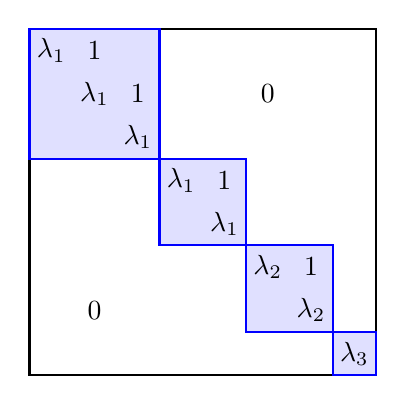
\begin{tikzpicture}[scale=0.55]
    % outer matrix
    \draw (0,0) rectangle (8,8);
    % block 1: J_3(lambda_1), top-left
    \fill[blue!12] (0,5) rectangle (3,8);
    \draw[thick, color=blue] (0,5) rectangle (3,8);
    \node at (0.5,7.5) {$\lambda_1$};
    \node at (1.5,7.5) {$1$};
    \node at (1.5,6.5) {$\lambda_1$};
    \node at (2.5,6.5) {$1$};
    \node at (2.5,5.5) {$\lambda_1$};
    % block 2: J_2(lambda_1)
    \fill[blue!12] (3,3) rectangle (5,5);
    \draw[thick, color=blue] (3,3) rectangle (5,5);
    \node at (3.5,4.5) {$\lambda_1$};
    \node at (4.5,4.5) {$1$};
    \node at (4.5,3.5) {$\lambda_1$};
    % block 3: J_2(lambda_2)
    \fill[blue!12] (5,1) rectangle (7,3);
    \draw[thick, color=blue] (5,1) rectangle (7,3);
    \node at (5.5,2.5) {$\lambda_2$};
    \node at (6.5,2.5) {$1$};
    \node at (6.5,1.5) {$\lambda_2$};
    % block 4: J_1(lambda_3)
    \fill[blue!12] (7,0) rectangle (8,1);
    \draw[thick, color=blue] (7,0) rectangle (8,1);
    \node at (7.5,0.5) {$\lambda_3$};
    % zero labels
    \node at (5.5,6.5) {$0$};
    \node at (1.5,1.5) {$0$};
\end{tikzpicture}
\end{center}
Note that repeated eigenvalues can appear in several different blocks (here $\lambda_1$ owns both a $3 \times 3$ and a $2 \times 2$ block).

The main theorem, which we will state but not prove\footnote{The proof is non-examinable, and follows from the structure theory of modules developed in IB Groups, Rings and Modules.}, is that this form can always be reached.

\begin{theorem}[Jordan Normal Form]
    Every matrix $A \in \mathcal{M}_{n,n}(\C)$ is similar to a matrix in Jordan normal form, which is unique up to reordering the Jordan blocks.
\end{theorem}

\begin{example}[JNF in Two Dimensions]
    Every $2 \times 2$ complex matrix is similar to exactly one of
    $$
    \begin{pmatrix}
        \lambda_1 & 0 \\ 0 & \lambda_2
    \end{pmatrix}, \qquad
    \begin{pmatrix}
        \lambda & 0 \\ 0 & \lambda
    \end{pmatrix}, \qquad
    \begin{pmatrix}
        \lambda & 1 \\ 0 & \lambda
    \end{pmatrix},
    $$
    with respective minimal polynomials $(t - \lambda_1)(t - \lambda_2)$, $(t - \lambda)$ and $(t - \lambda)^2$.
\end{example}

\subsection{Generalised Eigenspaces}

While we won't prove the Jordan normal form theorem in full, we can prove the decomposition of $V$ that underlies it. The idea is to relax the eigenspace condition $(\alpha - \lambda \operatorname{id})(v) = 0$, and instead only require that some \emph{power} of $(\alpha - \lambda\operatorname{id})$ kills $v$.

\begin{theorem}[Generalised Eigenspace Decomposition]
    Let $V$ be a finite dimensional $\C$-vector space and $\alpha$ an endomorphism of $V$ with minimal polynomial
    $$
    m_\alpha(t) = \prod_{j = 1}^k (t - \lambda_j)^{c_j},
    $$
    where the $\lambda_j$ are distinct. Then
    $$
    V = \bigoplus_{j = 1}^k V_j, \quad \text{where } V_j = \kernel\left((\alpha - \lambda_j\operatorname{id})^{c_j}\right)
    $$
    is called the \vocab{generalised eigenspace} associated to $\lambda_j$.
\end{theorem}
\begin{proof}
    The proof mirrors our diagonalisability criterion -- we construct explicit projections onto the pieces. Let
    $$
    p_j(t) = \prod_{i \neq j}(t - \lambda_i)^{c_i},
    $$
    so that $p_j (t)(t - \lambda_j)^{c_j} = m_\alpha(t)$. The polynomials $p_1, \dots, p_k$ have no common factor, so by the Euclidean algorithm there are polynomials $q_1, \dots, q_k$ with
    $$
    q_1 p_1 + \cdots + q_k p_k = 1.
    $$
    Define $\pi_j = (q_j p_j)(\alpha)$. Then immediately $\sum_j \pi_j = \operatorname{id}$, so every $v \in V$ decomposes as $v = \sum_j \pi_j(v)$; and each piece lies where it should, since
    $$
    (\alpha - \lambda_j \operatorname{id})^{c_j}\, \pi_j(v) = q_j(\alpha)\, m_\alpha(\alpha)(v) = 0,
    $$
    so $\pi_j(v) \in V_j$. Hence $V = \sum_j V_j$.

    For directness, note that if $i \neq j$ then $p_i p_j$ is divisible by $m_\alpha$, so $\pi_i \pi_j = 0$. Combining this with $\sum_j \pi_j = \operatorname{id}$ gives $\pi_i = \pi_i \left(\sum_j \pi_j\right) = \pi_i^2$, so each $\pi_i$ is a projection, and moreover $\pi_i$ acts as the identity on $V_i$ and as zero on $V_j$ for $j \neq i$.\footnote{To see $\pi_i$ acts as the identity on $V_i$: for $v \in V_i$, all the terms $\pi_j (v)$ with $j \neq i$ lie in $V_j$, and applying the identity $\operatorname{id} = \sum_j \pi_j$ twice with $\pi_i\pi_j = 0$ collapses everything except $\pi_i(v)$.} Then given any relation $v_1 + \cdots + v_k = 0$ with $v_j \in V_j$, applying $\pi_j$ picks out $v_j = 0$ for each $j$, so the sum is direct.
\end{proof}

\begin{remark}
    Each $V_j$ is stable under $\alpha$, and the restriction of $(\alpha - \lambda_j \operatorname{id})$ to $V_j$ is \emph{nilpotent} -- its $c_j$th power is zero. So the Jordan normal form theorem is really a statement about how nilpotent maps can act, and the $1$s above the diagonal record that nilpotent action.
\end{remark}

It's worth seeing concretely how a single Jordan block acts. Writing $J_m(\lambda) = \lambda I + N$, the basis vectors form a \emph{chain}: $N$ sends each basis vector to the previous one, eventually falling off the end into $0$.
\begin{center}
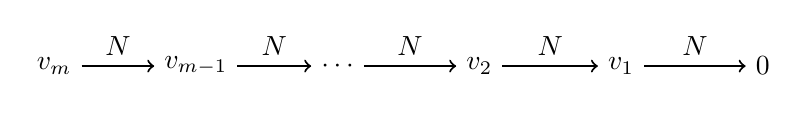
\begin{tikzpicture}[scale=1.0]
    \node (vm) at (0,0) {$v_m$};
    \node (vm1) at (1.8,0) {$v_{m-1}$};
    \node (dots) at (3.6,0) {$\cdots$};
    \node (v2) at (5.4,0) {$v_2$};
    \node (v1) at (7.2,0) {$v_1$};
    \node (z) at (9,0) {$0$};
    \draw[->] (vm) -- (vm1) node[midway, above] {$N$};
    \draw[->] (vm1) -- (dots) node[midway, above] {$N$};
    \draw[->] (dots) -- (v2) node[midway, above] {$N$};
    \draw[->] (v2) -- (v1) node[midway, above] {$N$};
    \draw[->] (v1) -- (z) node[midway, above] {$N$};
\end{tikzpicture}
\end{center}
Here $N = J_m(\lambda) - \lambda I$, and $N^k$ shifts the off-diagonal line of $1$s one step further from the diagonal each time, so $N^m = 0$ but $N^{m-1} \neq 0$.

This picture lets us read off all three multiplicities of an eigenvalue $\lambda$ directly from the Jordan normal form:
\begin{itemize}
    \item $a_\lambda$ is the \emph{total size} of all blocks with eigenvalue $\lambda$ (the number of times $\lambda$ appears on the diagonal),
    \item $g_\lambda$ is the \emph{number} of blocks with eigenvalue $\lambda$ (each block contributes exactly one independent eigenvector -- the start of its chain),
    \item $c_\lambda$ is the size of the \emph{largest} block with eigenvalue $\lambda$ (the longest chain takes the most steps to kill).
\end{itemize}
In particular, knowing $(a_\lambda, g_\lambda, c_\lambda)$ for each eigenvalue determines the Jordan normal form completely for small matrices, which makes computing it quite mechanical.

\subsection{Computing the Jordan Normal Form}

\begin{example}[Computing a JNF]
    Let's find the Jordan normal form of
    $$
    A = \begin{pmatrix}
        0 & -1 \\ 1 & 2
    \end{pmatrix},
    $$
    along with a basis realising it. The characteristic polynomial is $\chi_A(t) = t(2 - t) + 1 = (t-1)^2$, so $\lambda = 1$ is the only eigenvalue. Since $A - I \neq 0$, the minimal polynomial is $(t - 1)^2$, so $c_1 = 2$ and the JNF has a single $2 \times 2$ block:
    $$
    J = \begin{pmatrix}
        1 & 1 \\ 0 & 1
    \end{pmatrix}.
    $$
    To find the basis, we need a chain: a vector $v_2$ with $(A - I)v_2 = v_1 \neq 0$ and $(A - I)v_1 = 0$. We compute
    $$
    A - I = \begin{pmatrix}
        -1 & -1 \\ 1 & 1
    \end{pmatrix}, \quad \text{so} \quad \kernel(A - I) = \left\langle \begin{pmatrix} 1 \\ -1 \end{pmatrix} \right\rangle.
    $$
    Taking $v_1 = (1, -1)^T$, we then solve $(A - I)v_2 = v_1$, which gives (for example) $v_2 = (-1, 0)^T$. In the basis $\{v_1, v_2\}$ the map acts by $v_1 \mapsto v_1$ and $v_2 \mapsto v_1 + v_2$, so with $P = \begin{pmatrix} 1 & -1 \\ -1 & 0 \end{pmatrix}$ we have $A = PJP^{-1}$.
\end{example}

\section{Symmetric, Quadratic and Hermitian Forms}

We now return to bilinear forms, this time restricting our attention to forms $\phi: V \times V \rightarrow \F$ on a \emph{single} vector space. Just as we asked when an endomorphism can be represented by a diagonal matrix, we will ask when a bilinear form can -- and here the answer turns out to be much cleaner.

\subsection{Symmetric Bilinear Forms and Congruence}

For a bilinear form $\phi: V \times V \rightarrow \F$ and a basis $B$ of $V$, we write $[\phi]_B = [\phi]_{B, B}$. Specialising our change of basis result for bilinear forms, if $B'$ is another basis and $P = [I]_{B', B}$ is the change of basis matrix, then
$$
[\phi]_{B'} = P^T [\phi]_B P.
$$
This motivates the following analogue of similarity.

\begin{definition}[Congruent Matrices]
    Two square matrices $A, A' \in \mathcal{M}_{n,n}(\F)$ are \vocab{congruent} if $A' = P^T A P$ for some invertible matrix $P$.
\end{definition}

Congruence is an equivalence relation, and two matrices are congruent exactly when they represent the same bilinear form in different bases. So the question `when can $\phi$ be represented by a diagonal matrix?' is the question of classifying matrices up to congruence.

There is an immediate necessary condition. If $[\phi]_B = D$ is diagonal in some basis, then for any other basis, $[\phi]_{B'} = P^TDP$ satisfies $([\phi]_{B'})^T = P^T D^T P = [\phi]_{B'}$ -- the matrix of $\phi$ is symmetric in \emph{every} basis. This corresponds to a natural symmetry condition on the form itself.

\begin{definition}[Symmetric Bilinear Form]
    A bilinear form $\phi: V \times V \rightarrow \F$ is \vocab{symmetric} if $\phi(u, v) = \phi(v, u)$ for all $u, v \in V$.
\end{definition}

It's easy to check that $\phi$ is symmetric if and only if $[\phi]_B$ is a symmetric matrix for any (equivalently, every) basis $B$. Remarkably, this necessary condition for diagonalisability turns out to be sufficient, as we will prove shortly.

\subsection{Quadratic Forms}

Before that, let's meet the closely-related notion of a \emph{quadratic form}, which is what you get when you feed a bilinear form the same vector twice.

\begin{definition}[Quadratic Form]
    A map $Q: V \rightarrow \F$ is a \vocab{quadratic form} if there is some bilinear form $\phi: V \times V \rightarrow \F$ with
    $$
    Q(v) = \phi(v, v) \text{ for all } v \in V.
    $$
\end{definition}

In coordinates, if $[\phi]_B = A$ and $x = [v]_B$, then $Q(v) = x^T A x$ is a homogeneous quadratic polynomial in the coordinates of $v$ -- hence the name. Note that
$$
x^T A x = \sum_{i,j} a_{ij}x_i x_j = \sum_{i, j} \frac{a_{ij} + a_{ji}}{2} x_i x_j = x^T \left(\frac{A + A^T}{2}\right) x,
$$
so we lose nothing by assuming the underlying matrix is symmetric. This observation upgrades to a bijection between quadratic forms and symmetric bilinear forms.

\begin{proposition}[Polarisation Identity]
    Let $Q: V \rightarrow \F$ be a quadratic form (where the characteristic of $\F$ is not $2$). Then there is a \emph{unique} symmetric bilinear form $\phi$ with $Q(v) = \phi(v, v)$, given by
    $$
    \phi(u, v) = \frac{1}{2}\left(Q(u + v) - Q(u) - Q(v)\right).
    $$
\end{proposition}
\begin{proof}
    For existence, take any bilinear $\psi$ with $Q(v) = \psi(v,v)$ and symmetrise: $\phi(u, v) = \frac{1}{2}(\psi(u,v) + \psi(v, u))$ is symmetric, bilinear, and has $\phi(v,v) = \psi(v,v) = Q(v)$.

    For uniqueness, if $\phi$ is any symmetric bilinear form representing $Q$, then expanding gives
    $$
    Q(u + v) = \phi(u + v, u + v) = Q(u) + Q(v) + 2\phi(u, v),
    $$
    so $\phi$ is determined by $Q$ via the stated formula.
\end{proof}

So symmetric bilinear forms and quadratic forms are two views of the same data, and we can pass between them freely.

\subsection{Diagonalising Symmetric Bilinear Forms}

\begin{theorem}[Diagonalisability of Symmetric Bilinear Forms]
    Let $\phi: V \times V \rightarrow \F$ be a symmetric bilinear form on a finite dimensional vector space $V$. Then there is a basis $B$ of $V$ such that $[\phi]_B$ is diagonal.
\end{theorem}
\begin{proof}
    We induct on $n = \dim V$, the case $n \leq 1$ being trivial. If $\phi(v, v) = 0$ for every $v \in V$, then by the polarisation identity $\phi = 0$, which is certainly diagonal. Otherwise, pick $e_1$ with $\phi(e_1, e_1) \neq 0$, and let
    $$
    U = \{v \in V \mid \phi(e_1, v) = 0\},
    $$
    the kernel of the linear map $v \mapsto \phi(e_1, v)$. This map is a non-zero element of $V^*$ (it doesn't vanish at $e_1$), so by rank-nullity $\dim U = n - 1$. Moreover $\langle e_1 \rangle \cap U = \{0\}$, since $\lambda e_1 \in U$ forces $\lambda \phi(e_1, e_1) = 0$, so $\lambda = 0$. Counting dimensions, $V = \langle e_1 \rangle \oplus U$.

    By induction, the restriction $\phi|_{U \times U}$ is diagonal in some basis $\{e_2, \dots, e_n\}$ of $U$. Then in the basis $B = \{e_1, e_2, \dots, e_n\}$, using symmetry and $\phi(e_1, e_j) = 0$ for $j \geq 2$, the matrix $[\phi]_B$ is diagonal.
\end{proof}

The proof is really an algorithm, but in practice there's often a faster route: \emph{completing the square}.

\begin{example}[Diagonalising by Completing the Square]
    Consider the quadratic form on $\R^3$ given by
    $$
    Q(x_1, x_2, x_3) = x_1^2 + x_2^2 + 2x_3^2 + 2x_1x_2 + 2x_1 x_3 - 2x_2x_3,
    $$
    corresponding to the symmetric matrix
    $$
    A = \begin{pmatrix}
        1 & 1 & 1 \\
        1 & 1 & -1 \\
        1 & -1 & 2
    \end{pmatrix}
    $$
    (note the off-diagonal entries are \emph{half} the corresponding coefficients, since each cross term appears twice in $x^TAx$). Gathering every appearance of $x_1$ into a single square, we compute
    $$
    Q - (x_1 + x_2 + x_3)^2 = x_3^2 - 4x_2 x_3,
    $$
    and then completing the square again in $x_3$,
    \begin{align*}
        Q &= (x_1 + x_2 + x_3)^2 + x_3^2 - 4x_2x_3 \\
        &= (x_1 + x_2 + x_3)^2 + (x_3 - 2x_2)^2 - 4x_2^2.
    \end{align*}
    So in the new coordinates $x_1' = x_1 + x_2 + x_3$, $x_2' = x_3 - 2x_2$, $x_3' = 2x_2$, we have $Q = x_1'^2 + x_2'^2 - x_3'^2$, and the form is diagonal with diagonal entries $1, 1, -1$.
\end{example}

\subsection{Sylvester's Law of Inertia}

Over $\C$, we can go further than just `diagonal': dividing each basis vector $e_i$ by a square root of $\phi(e_i, e_i)$, every non-zero diagonal entry can be scaled to $1$.

\begin{corollary}[Canonical Form over $\C$]
    Let $\phi$ be a symmetric bilinear form on a finite dimensional $\C$-vector space $V$. Then there is a basis $B$ with
    $$
    [\phi]_B = \left(\begin{array}{ c | c }
        I_r & 0 \\
        \hline
        0 & 0
      \end{array}\right),
    $$
    where $r = r(\phi)$. Equivalently, every complex symmetric matrix is congruent to exactly one matrix of this form.
\end{corollary}

Over $\R$ we cannot take square roots of negative numbers, so the best we can do is scale each non-zero diagonal entry to $\pm 1$.

\begin{corollary}[Canonical Form over $\R$]
    Let $\phi$ be a symmetric bilinear form on a finite dimensional $\R$-vector space $V$. Then there is a basis $B$ with
    $$
    [\phi]_B = \begin{pmatrix}
        I_p & & \\
        & -I_q & \\
        & & 0
    \end{pmatrix}
    $$
    for some non-negative integers $p, q$ with $p + q = r(\phi)$.
\end{corollary}
\begin{proof}
    Diagonalise $\phi$, reorder the basis so the positive diagonal entries $a_1, \dots, a_p$ come first, then the negative entries $a_{p + 1}, \dots, a_{p+q}$, then the zeros, and replace $e_i$ by $e_i / \sqrt{|a_i|}$ for $i \leq p + q$.
\end{proof}

In terms of the associated quadratic form, this says that after a linear change of coordinates, any real quadratic form looks like
$$
Q(x) = x_1^2 + \cdots + x_p^2 - x_{p+1}^2 - \cdots - x_{p + q}^2,
$$
where $p$ directions count positively, $q$ count negatively, and the rest are invisible to $Q$.
\begin{center}
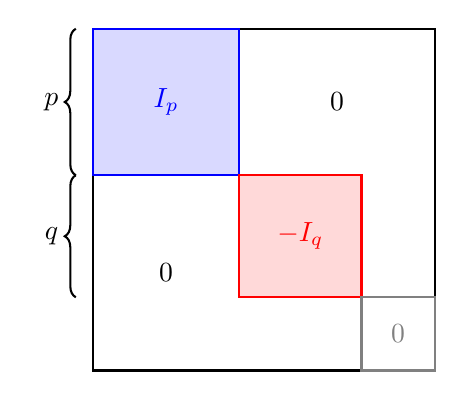
\begin{tikzpicture}[scale=0.62]
    \draw (0,0) rectangle (7,7);
    \fill[blue!15] (0,4) rectangle (3,7);
    \draw[thick, color=blue] (0,4) rectangle (3,7);
    \node[color=blue] at (1.5,5.5) {$I_p$};
    \fill[red!15] (3,1.5) rectangle (5.5,4);
    \draw[thick, color=red] (3,1.5) rectangle (5.5,4);
    \node[color=red] at (4.25,2.75) {$-I_q$};
    \draw[thick, color=gray] (5.5,0) rectangle (7,1.5);
    \node[color=gray] at (6.25,0.75) {$0$};
    \node at (5,5.5) {$0$};
    \node at (1.5,2) {$0$};
    \draw[decorate, decoration={brace, amplitude=4pt}] (-0.35,4) -- (-0.35,7) node[midway, left, inner sep=6pt] {$p$};
    \draw[decorate, decoration={brace, amplitude=4pt}] (-0.35,1.5) -- (-0.35,4) node[midway, left, inner sep=6pt] {$q$};
\end{tikzpicture}
\end{center}
The remarkable fact -- \emph{Sylvester's law of inertia} -- is that the numbers $p$ and $q$ do not depend on how you diagonalised.

\begin{theorem}[Sylvester's Law of Inertia]
    Let $\phi$ be a symmetric bilinear form on a finite dimensional real vector space $V$. If $\phi$ is represented by the matrix above with parameters $(p, q)$ in one basis and $(p', q')$ in another, then $p = p'$ and $q = q'$.
\end{theorem}

\begin{definition}[Signature]
    The \vocab{signature} of a real symmetric bilinear form $\phi$ is $s(\phi) = p - q$.
\end{definition}

To prove Sylvester's law, we need a basis-independent characterisation of $p$, and the right notion is the following.

\begin{definition}[Definiteness]
    A symmetric bilinear form $\phi$ on a real vector space $V$ is:
    \begin{enumerate}[label=(\roman*)]
        \item \vocab{positive definite} if $\phi(v, v) > 0$ for all $v \neq 0$,
        \item \vocab{positive semi-definite} if $\phi(v,v) \geq 0$ for all $v \in V$,
    \end{enumerate}
    with \vocab{negative (semi-)definite} defined analogously with the inequalities reversed.
\end{definition}

\begin{proof}[Proof of Sylvester's Law]
    Suppose $B = \{v_1, \dots, v_n\}$ is a basis in which $[\phi]_B$ has the canonical form with parameters $(p, q)$. We claim
    $$
    p = \max \{\dim X \mid X \leq V, \; \phi|_{X \times X} \text{ positive definite}\},
    $$
    which is manifestly basis-independent, so proves that $p$ (and by the same argument applied to $-\phi$, also $q$) is well defined.

    First, $\phi$ restricted to $X_0 = \langle v_1, \dots, v_p \rangle$ is positive definite, so the maximum is at least $p$. Conversely, let $Y = \langle v_{p +1}, \dots, v_n\rangle$, on which $\phi$ is negative semi-definite, and suppose $X'$ is any subspace on which $\phi$ is positive definite. Then $X' \cap Y = \{0\}$, since any $v$ in the intersection has $\phi(v,v) > 0$ and $\phi(v,v) \leq 0$ unless $v = 0$. Hence the sum $X' + Y$ is direct, and
    $$
    \dim X' + (n - p) = \dim X' + \dim Y \leq \dim V = n,
    $$
    giving $\dim X' \leq p$ as required.
\end{proof}

\begin{remark}
    Since $p + q = r(\phi)$ is the rank, and $(p, q)$ determine the canonical form completely, we get a tidy classification: two real symmetric matrices are congruent if and only if they have the same rank and signature.
\end{remark}

\subsection{Sesquilinear and Hermitian Forms}

Over $\C$, symmetric bilinear forms are not quite the right notion for measuring `length'. The problem is visible even in one dimension: for the form $\phi(x, y) = xy$ on $\C$, we get $\phi(ix, ix) = -\phi(x,x)$, so no non-zero form of this kind takes only real positive values. The fix is to build in a complex conjugate.

\begin{definition}[Sesquilinear Form]
    Let $V, W$ be $\C$-vector spaces. A map $\phi: V \times W \rightarrow \C$ is \vocab{sesquilinear} if it is linear in the first argument and \emph{antilinear} in the second, meaning
    $$
    \phi(v, \lambda_1 w_1 + \lambda_2 w_2) = \overline{\lambda_1}\phi(v, w_1) + \overline{\lambda_2}\phi(v, w_2).
    $$
\end{definition}

The matrix theory carries over with only cosmetic changes: with respect to bases $B$ of $V$ and $C$ of $W$, we define $([\phi]_{B, C})_{ij} = \phi(v_i, w_j)$ as before, and then
$$
\phi(v, w) = [v]_B^T \, [\phi]_{B,C}\, \overline{[w]_C}, \qquad [\phi]_{B', C'} = P^T [\phi]_{B, C} \overline{Q}
$$
for change of basis matrices $P, Q$.

The analogue of a symmetric form is the following.

\begin{definition}[Hermitian Form]
    A sesquilinear form $\phi: V \times V \rightarrow \C$ is \vocab{Hermitian} if
    $$
    \phi(u, v) = \overline{\phi(v, u)} \quad \text{for all } u, v \in V.
    $$
\end{definition}

Note that for a Hermitian form, $\phi(v, v) = \overline{\phi(v,v)}$ is always \emph{real} -- which is what makes definiteness meaningful over $\C$ -- and $\phi(\lambda v, \lambda v) = |\lambda|^2 \phi(v,v)$, so scaling can't change signs as it did above.

\begin{lemma}[Matrix Criterion for Hermitian Forms]
    A sesquilinear form $\phi$ on $V$ is Hermitian if and only if for any basis $B$ of $V$,
    $$
    [\phi]_B = \overline{[\phi]_B}^T =: [\phi]_B^\dagger.
    $$
\end{lemma}
\begin{proof}
    If $\phi$ is Hermitian, then $a_{ji} = \phi(v_j, v_i) = \overline{\phi(v_i, v_j)} = \overline{a_{ij}}$. Conversely, if $A = A^\dagger$, then expanding $u = \sum_i \lambda_i v_i$ and $v = \sum_j \mu_j v_j$ gives
    $$
    \phi(u, v) = \sum_{i, j}\lambda_i \overline{\mu_j} a_{ij}, \qquad \overline{\phi(v, u)} = \overline{\sum_{i,j} \mu_j \overline{\lambda_i} a_{ji}} = \sum_{i,j} \lambda_i \overline{\mu_j}\, \overline{a_{ji}},
    $$
    and these agree since $\overline{a_{ji}} = a_{ij}$.
\end{proof}

There is also a Hermitian version of polarisation, this time requiring four terms:
$$
\phi(u, v) = \frac{1}{4}\left(Q(u + v) - Q(u - v) + iQ(u + iv) - iQ(u - iv)\right),
$$
where $Q(v) = \phi(v,v)$. So again, a Hermitian form is entirely determined by the real-valued function $Q$.

Sylvester's law then goes through essentially verbatim.

\begin{theorem}[Sylvester's Law for Hermitian Forms]
    Let $\phi$ be a Hermitian form on a finite dimensional $\C$-vector space $V$. Then there is a basis $B$ of $V$ in which
    $$
    [\phi]_B = \begin{pmatrix}
        I_p & & \\
        & -I_q & \\
        & & 0
    \end{pmatrix},
    $$
    and the integers $p$ and $q$ depend only on $\phi$, not on the basis.
\end{theorem}
\begin{proof}[Proof Sketch]
    Existence follows the real symmetric case: if $\phi \neq 0$, polarisation gives some $e_1$ with $\phi(e_1, e_1) \neq 0$ (a real number), we normalise so that $\phi(v_1, v_1) = \pm 1$, split off $\langle v_1 \rangle^\perp$ using rank-nullity, and induct. Uniqueness follows Sylvester's law: $p$ is again the maximal dimension of a subspace on which $\phi$ is positive definite, which makes sense as $\phi(v,v)$ is real.
\end{proof}

\subsection{Skew-Symmetric Forms}

For completeness, let us briefly mention the opposite symmetry class. A bilinear form $\phi$ on a real vector space is \vocab{skew-symmetric} if $\phi(u, v) = -\phi(v, u)$ for all $u, v$, or equivalently if its matrix satisfies $A = -A^T$ in any basis. Note that any bilinear form decomposes as a sum of a symmetric and a skew-symmetric form, via
$$
\phi(u,v) = \underbrace{\frac{\phi(u,v) + \phi(v,u)}{2}}_{\text{symmetric}} + \underbrace{\frac{\phi(u,v) - \phi(v,u)}{2}}_{\text{skew-symmetric}}.
$$

\begin{theorem}[Canonical Form for Skew-Symmetric Forms]
    Let $\phi$ be a skew-symmetric bilinear form on a finite dimensional real vector space $V$. Then there is a basis $B = \{v_1, w_1, \dots, v_m, w_m, v_{2m + 1}, \dots, v_n\}$ in which $[\phi]_B$ is block diagonal, beginning with $m$ blocks of the form
    $$
    \begin{pmatrix}
        0 & 1 \\ -1 & 0
    \end{pmatrix}
    $$
    followed by zeros. In particular, a skew-symmetric matrix has even rank.
\end{theorem}
\begin{proof}[Proof Sketch]
    If $\phi \neq 0$, pick $v_1, w_1$ with $\phi(v_1, w_1) = 1$ (rescaling as needed); skew-symmetry gives $\phi(w_1, v_1) = -1$, and $v_1, w_1$ are independent since $\phi(v, v) = 0$ for every $v$. Set $U = \langle v_1, w_1 \rangle$ and let $W = \{v \in V \mid \phi(v_1, v) = \phi(w_1, v) = 0\}$. A dimension count shows $V = U \oplus W$, and we induct on $W$.
\end{proof}

\section{Inner Product Spaces}

In this final section we add the last piece of structure to our vector spaces: a notion of \emph{length} and \emph{angle}. All of the geometry that this makes possible comes from a single piece of data -- an inner product -- and the positive-definite forms of the previous section are exactly what we need. Throughout this section, $V$ is a vector space over $\R$ or $\C$.

\subsection{Inner Products}

\begin{definition}[Inner Product]
    An \vocab{inner product} on $V$ is a positive definite symmetric bilinear form (if $V$ is a real vector space) or positive definite Hermitian sesquilinear form (if $V$ is complex). We write $\phi(u, v) = \langle u, v\rangle$, and call $V$ equipped with an inner product an \vocab{inner product space}.
\end{definition}

\begin{example}[Examples of Inner Products]~
    \vspace{-1.5\baselineskip}
    \begin{enumerate}[label=(\roman*)]
        \item On $\R^n$, the familiar dot product $\langle x, y \rangle = \sum_{i = 1}^n x_i y_i$; on $\C^n$, the standard inner product $\langle x, y \rangle = \sum_{i = 1}^n x_i \overline{y_i}$.
        \item On $\mathcal{C}([0,1], \C)$, the \emph{$L^2$ inner product}
        $$
        \langle f, g \rangle = \int_0^1 f(t)\overline{g(t)} \dd t.
        $$
        \item More generally, given a continuous `weight' function $w: [0, 1] \rightarrow \R_{> 0}$, we can define $\langle f, g\rangle = \int_0^1 f(t)\overline{g(t)}w(t) \dd t$.
    \end{enumerate}
\end{example}

When checking that something is an inner product, linearity and symmetry are usually immediate, and the only real content is positive definiteness -- often just the statement that $\langle v, v \rangle = 0$ implies $v = 0$.

\begin{definition}[Norm]
    Let $V$ be an inner product space. The \vocab{norm} of $v \in V$ is
    $$
    \norm{v} = \sqrt{\langle v, v\rangle},
    $$
    which is a non-negative real number, and is zero only for $v = 0$.
\end{definition}

The single most useful inequality relating the norm and the inner product is the following.

\begin{theorem}[Cauchy-Schwarz Inequality]
    Let $V$ be an inner product space, and $u, v \in V$. Then
    $$
    |\langle u, v \rangle| \leq \norm{u} \norm{v}.
    $$
\end{theorem}
\begin{proof}
    If $u = 0$ the result is trivial, so assume $u \neq 0$. For any scalar $t$, positive definiteness gives
    $$
    0 \leq \norm{tu - v}^2 = |t|^2 \norm{u}^2 - 2\re\left(t \langle u, v\rangle\right) + \norm{v}^2.
    $$
    Choosing $t = \overline{\langle u, v\rangle}/\norm{u}^2$ (the choice that makes the bound tightest), the right hand side becomes
    $$
    \frac{|\langle u, v\rangle|^2}{\norm{u}^2} - 2\frac{|\langle u, v\rangle|^2}{\norm{u}^2} + \norm{v}^2 = \norm{v}^2 - \frac{|\langle u, v\rangle|^2}{\norm{u}^2} \geq 0,
    $$
    which rearranges to the desired inequality.
\end{proof}

\begin{corollary}[Triangle Inequality]
    In an inner product space, $\norm{u + v} \leq \norm{u} + \norm{v}$.
\end{corollary}
\begin{proof}
    Expanding and applying Cauchy-Schwarz,
    $$
    \norm{u + v}^2 = \norm{u}^2 + 2\re \langle u, v\rangle + \norm{v}^2 \leq \norm{u}^2 + 2\norm{u}\norm{v} + \norm{v}^2 = (\norm{u} + \norm{v})^2. \qedhere
    $$
\end{proof}

\subsection{Orthogonality}

\begin{definition}[Orthogonal and Orthonormal Sets]
    A set $\{e_1, \dots, e_k\}$ of vectors in an inner product space is \vocab{orthogonal} if $\langle e_i, e_j \rangle = 0$ for all $i \neq j$, and \vocab{orthonormal} if additionally $\norm{e_i} = 1$ for each $i$, so that $\langle e_i, e_j \rangle = \delta_{ij}$.
\end{definition}

Orthogonality is a strong condition -- strong enough to give linear independence for free, along with an explicit formula for coordinates.

\begin{lemma}[Orthogonality Implies Independence]
    Let $\{e_1, \dots, e_k\}$ be orthogonal non-zero vectors. Then they are linearly independent, and if $v = \sum_{j = 1}^k \lambda_j e_j$ then
    $$
    \lambda_j = \frac{\langle v, e_j \rangle}{\norm{e_j}^2}.
    $$
\end{lemma}
\begin{proof}
    Taking the inner product of $v = \sum_i \lambda_i e_i$ with $e_j$, all terms with $i \neq j$ vanish, leaving $\langle v, e_j \rangle = \lambda_j \norm{e_j}^2$, which gives the coordinate formula. In particular if $v = 0$ then every $\lambda_j = 0$, which is linear independence.
\end{proof}

For orthonormal \emph{bases} the coordinate formula becomes $\lambda_j = \langle v, e_j\rangle$, and the inner product itself takes a particularly clean coordinate form.

\begin{corollary}[Parseval's Identity]
    Let $V$ be a finite dimensional inner product space with orthonormal basis $\{e_1, \dots, e_n\}$. Then for all $u, v \in V$,
    $$
    \langle u, v \rangle = \sum_{i = 1}^n \langle u, e_i \rangle \overline{\langle v, e_i\rangle}, \quad \text{and in particular} \quad \norm{u}^2 = \sum_{i = 1}^n |\langle u, e_i \rangle|^2.
    $$
\end{corollary}
\begin{proof}
    Expand $u = \sum_i \langle u, e_i\rangle e_i$ and $v = \sum_j \langle v, e_j \rangle e_j$ and use sesquilinearity together with $\langle e_i, e_j \rangle = \delta_{ij}$. The second identity is the case $u = v$.
\end{proof}

\subsection{The Gram-Schmidt Process}

Orthonormal bases are clearly a pleasant thing to have, and happily there is an algorithm that manufactures them from arbitrary bases: the \emph{Gram-Schmidt process}. The idea of each step is simple -- subtract off the components of the next vector lying along the directions already constructed, then rescale what's left.

\begin{center}
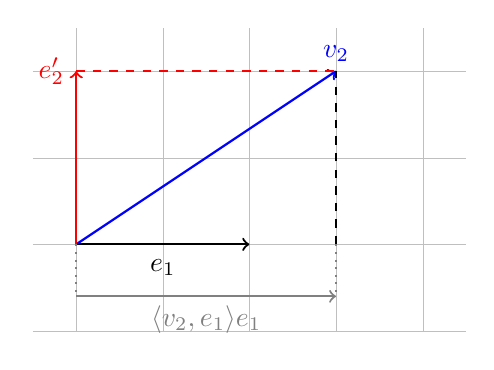
\begin{tikzpicture}[scale=1.1]
    \draw[ultra thin, color=lightgray] (-0.5,-1.0) grid (4.5,2.5);
    \draw[->, thick] (0,0) -- (2,0) node[pos=0.5, below, inner sep=5pt] {$e_1$};
    \draw[->, thick, color=blue] (0,0) -- (3,2) node[above, inner sep=3pt] {$v_2$};
    \draw[dashed] (3,0) -- (3,2);
    \draw[->, thick, color=red] (0,0) -- (0,2) node[left, inner sep=4pt] {$e_2'$};
    \draw[dashed, color=red] (0,2) -- (3,2);
    \draw[->, color=gray] (0,-0.6) -- (3,-0.6);
    \draw[dotted, color=gray] (0,0) -- (0,-0.6);
    \draw[dotted, color=gray] (3,0) -- (3,-0.6);
    \node[color=gray, below, inner sep=3pt] at (1.5,-0.6) {$\langle v_2, e_1\rangle e_1$};
\end{tikzpicture}
\end{center}

\begin{theorem}[Gram-Schmidt Orthogonalisation]
    Let $V$ be an inner product space, and let $v_1, v_2, \dots$ be a (finite or countable) linearly independent family of vectors. Then there is an orthonormal family $e_1, e_2, \dots$ such that for every $k$,
    $$
    \langle v_1, \dots, v_k \rangle = \langle e_1, \dots, e_k \rangle.
    $$
\end{theorem}
\begin{proof}
    We construct the $e_i$ inductively. To start, take $e_1 = v_1/\norm{v_1}$. Now suppose $e_1, \dots, e_k$ have been constructed, orthonormal and spanning $\langle v_1, \dots, v_k\rangle$. Define
    $$
    e_{k+1}' = v_{k + 1} - \sum_{i = 1}^k \langle v_{k+1}, e_i \rangle e_i.
    $$
    For each $j \leq k$ we then have
    $$
    \langle e_{k+1}', e_j \rangle = \langle v_{k + 1}, e_j\rangle - \langle v_{k+1}, e_j \rangle = 0,
    $$
    so $e_{k+1}'$ is orthogonal to everything so far. It is also non-zero, since otherwise $v_{k+1}$ would lie in $\langle e_1, \dots, e_k \rangle = \langle v_1, \dots, v_k\rangle$, contradicting linear independence. So we can set $e_{k+1} = e_{k+1}'/\norm{e_{k+1}'}$, and the spans match up since $e_{k + 1}$ is a linear combination of $v_{k+1}$ and $e_1, \dots, e_k$ (and vice versa).
\end{proof}

\begin{corollary}[Orthonormal Bases Exist]
    Every finite dimensional inner product space has an orthonormal basis, and any orthonormal set of vectors can be extended to an orthonormal basis.
\end{corollary}
\begin{proof}
    Apply Gram-Schmidt to any basis for the first claim. For the second, extend the orthonormal set to any basis and apply Gram-Schmidt -- the process leaves the already-orthonormal initial vectors unchanged.
\end{proof}

Interpreting Gram-Schmidt through matrices gives a classical matrix factorisation.

\begin{definition}[Orthogonal and Unitary Matrices]
    A matrix $A \in \mathcal{M}_{n,n}(\R)$ is \vocab{orthogonal} if $A^TA = I$, that is $A^{-1} = A^T$. A matrix $A \in \mathcal{M}_{n,n}(\C)$ is \vocab{unitary} if $A^\dagger A = I$, that is $A^{-1} = A^\dagger = \overline{A}^T$.
\end{definition}

Note that $A$ is orthogonal (or unitary) precisely when its columns form an orthonormal basis of $\F^n$ with the standard inner product.

\begin{proposition}[QR Decomposition]
    Every invertible matrix $A \in \mathcal{M}_{n,n}(\R)$ (respectively $\C$) can be written as $A = QR$ with $Q$ orthogonal (respectively unitary) and $R$ upper triangular.
\end{proposition}
\begin{proof}[Proof Sketch]
    Apply Gram-Schmidt to the columns $v_1, \dots, v_n$ of $A$, producing an orthonormal basis $e_1, \dots, e_n$. By construction each $v_k$ is a linear combination of $e_1, \dots, e_k$ only, so the matrix $Q$ with columns $e_i$ satisfies $A = QR$ with $R$ upper triangular.
\end{proof}

\subsection{Orthogonal Complements and Projections}

\begin{definition}[Orthogonal Complement]
    Let $V$ be an inner product space and $W \leq V$. The \vocab{orthogonal complement} of $W$ is
    $$
    W^\perp = \{ v \in V \mid \langle v, w \rangle = 0 \text{ for all } w \in W\}.
    $$
\end{definition}

\begin{lemma}[Orthogonal Decomposition]
    Let $V$ be a finite dimensional inner product space and $W \leq V$. Then $V = W \oplus W^\perp$.
\end{lemma}
\begin{proof}
    If $v \in W \cap W^\perp$ then $\norm{v}^2 = \langle v, v \rangle = 0$, so the intersection is trivial. For the sum, take an orthonormal basis $\{e_1, \dots, e_k\}$ of $W$ and extend it to an orthonormal basis $\{e_1, \dots, e_n\}$ of $V$; then $e_{k + 1}, \dots, e_n \in W^\perp$, so $W + W^\perp$ contains a basis of $V$.
\end{proof}

Compare this with the general situation for direct complements: earlier we emphasised that a subspace has \emph{many} complements, with no way to prefer one. An inner product fixes this -- $W^\perp$ is a \emph{canonical} complement.

Whenever $V = U \oplus W$, we can define the \vocab{projection} $\pi: V \rightarrow V$ onto $W$ by writing $v = u + w$ uniquely and setting $\pi(v) = w$; this is linear and satisfies $\pi^2 = \pi$. When the decomposition is the orthogonal one, $\pi$ has a beautiful geometric property: it finds the \emph{closest point} of $W$.

\begin{center}
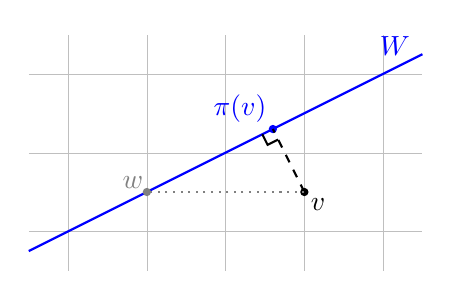
\begin{tikzpicture}[scale=1.0]
    \draw[ultra thin, color=lightgray] (-0.5,-0.5) grid (4.5,2.5);
    \draw[thick, color=blue] (-0.5,-0.25) -- (4.5,2.25);
    \node[color=blue] at (4.15,2.35) {$W$};
    \fill (3,0.5) circle (1.5pt) node[below right, inner sep=2pt] {$v$};
    \fill[color=blue] (2.6,1.3) circle (1.5pt) node[above left, inner sep=2pt, color=blue] {$\pi(v)$};
    \draw[dashed] (3,0.5) -- (2.6,1.3);
    \fill[color=gray] (1.0,0.5) circle (1.5pt) node[above left, inner sep=1pt, color=gray] {$w$};
    \draw[dotted, color=gray] (3,0.5) -- (1.0,0.5);
    % right angle marker at pi(v)
    \draw (2.466,1.233) -- (2.533,1.099) -- (2.667,1.166);
\end{tikzpicture}
\end{center}

\begin{proposition}[Orthogonal Projection is the Closest Point]
    Let $V$ be an inner product space and $W \leq V$ a finite dimensional subspace with orthonormal basis $\{e_1, \dots, e_k\}$. Define
    $$
    \pi(v) = \sum_{i = 1}^k \langle v, e_i \rangle e_i.
    $$
    Then $\pi$ is the projection onto $W$ along $W^\perp$, and for every $w \in W$,
    $$
    \norm{v - \pi(v)} \leq \norm{v - w},
    $$
    with equality if and only if $w = \pi(v)$. That is, $\pi(v)$ is the unique closest point of $W$ to $v$.
\end{proposition}
\begin{proof}
    Certainly $\pi(v) \in W$. Moreover $v - \pi(v) \in W^\perp$, since for each basis vector $e_j$,
    $$
    \langle v - \pi(v), e_j \rangle = \langle v, e_j \rangle - \sum_{i = 1}^k \langle v, e_i \rangle \langle e_i, e_j \rangle = \langle v, e_j\rangle - \langle v, e_j \rangle = 0.
    $$
    So $v = (v - \pi(v)) + \pi(v)$ is exactly the decomposition of $v$ with respect to $V = W^\perp \oplus W$, and $\pi$ is the claimed projection.

    For the closest point property, let $w \in W$ and split $v - w$ into orthogonal pieces:
    $$
    \norm{v - w}^2 = \norm{\underbrace{(v - \pi(v))}_{\in W^\perp} + \underbrace{(\pi(v) - w)}_{\in W}}^2 = \norm{v - \pi(v)}^2 + \norm{\pi(v) - w}^2,
    $$
    where the cross terms vanish by orthogonality (this is just Pythagoras). The right hand side is minimised exactly when $\pi(v) = w$.
\end{proof}

\subsection{Adjoint Maps}

We come now to the inner product space analogue of the dual map.

\begin{theorem}[Existence of the Adjoint]
    Let $V, W$ be finite dimensional inner product spaces and let $\alpha: V \rightarrow W$ be a linear map. Then there is a unique linear map $\alpha^*: W \rightarrow V$, the \vocab{adjoint} of $\alpha$, such that
    $$
    \langle \alpha(v), w \rangle = \langle v, \alpha^*(w)\rangle \quad \text{for all } v \in V,\; w \in W.
    $$
    Moreover, if $B$ and $C$ are \emph{orthonormal} bases of $V$ and $W$, then
    $$
    [\alpha^*]_{C, B} = [\alpha]_{B,C}^\dagger,
    $$
    the conjugate transpose of the matrix of $\alpha$.
\end{theorem}
\begin{proof}
    Let $B = \{v_1, \dots, v_n\}$, $C = \{w_1, \dots, w_m\}$ be orthonormal bases, and let $A = [\alpha]_{B, C}$. Define $\alpha^*$ to be the linear map with matrix $[\alpha^*]_{C,B} = A^\dagger$. Then for basis vectors, using orthonormality to compute inner products,
    $$
    \langle \alpha(v_i), w_j \rangle = \left\langle \sum_{k} a_{ki} w_k, w_j \right\rangle = a_{ji}, \qquad
    \langle v_i, \alpha^*(w_j) \rangle = \left\langle v_i, \sum_k \overline{a_{jk}} v_k \right\rangle = \overline{\overline{a_{ji}}} = a_{ji},
    $$
    and by (sesqui)linearity the two sides agree for all vectors. For uniqueness, if $\beta$ also satisfies the defining property then $\langle v, (\alpha^* - \beta)(w)\rangle = 0$ for all $v$, and taking $v = (\alpha^* - \beta)(w)$ shows $(\alpha^* - \beta)(w) = 0$ for every $w$.
\end{proof}

\begin{remark}
    We are recycling the notation $\alpha^*$ from dual maps, and this is no accident. The inner product gives an (antilinear) identification $v \mapsto \langle \cdot\,, v \rangle$ of $V$ with $V^*$, and under this identification the adjoint \emph{is} the dual map. This is also why the matrix of the adjoint is a (conjugate) transpose, just as the matrix of the dual map was a transpose.
\end{remark}

\subsection{Self-Adjoint Maps and Isometries}

Two classes of endomorphisms of an inner product space deserve special attention -- those that equal their own adjoint, and those whose adjoint is their inverse.

\begin{definition}[Self-Adjoint and Isometric Maps]
    Let $V$ be a finite dimensional inner product space, and let $\alpha: V \rightarrow V$ be an endomorphism.
    \begin{enumerate}[label=(\roman*)]
        \item $\alpha$ is \vocab{self-adjoint} if $\alpha^* = \alpha$, that is, $\langle \alpha(v), w \rangle = \langle v, \alpha(w)\rangle$ for all $v, w$. Over $\R$ such maps are called \vocab{symmetric}; over $\C$, \vocab{Hermitian}.
        \item $\alpha$ is an \vocab{isometry} if $\alpha^* = \alpha^{-1}$, or equivalently $\langle \alpha(v), \alpha(w)\rangle = \langle v, w \rangle$ for all $v, w$. Over $\R$ such maps are called \vocab{orthogonal}; over $\C$, \vocab{unitary}.
    \end{enumerate}
\end{definition}

Let's check the claimed equivalence for isometries. If $\alpha$ preserves all inner products, then in particular $\norm{\alpha(v)} = \norm{v}$, so $\alpha$ is injective, hence invertible; and then
$$
\langle v, \alpha^*(w)\rangle = \langle \alpha(v), w \rangle = \langle \alpha(v), \alpha(\alpha^{-1}(w))\rangle = \langle v, \alpha^{-1}(w)\rangle
$$
for all $v, w$, forcing $\alpha^* = \alpha^{-1}$. The converse is immediate: $\langle \alpha(v), \alpha(w)\rangle = \langle v, \alpha^*\alpha(w)\rangle = \langle v, w \rangle$. In fact, by polarisation, preserving norms alone is enough to make $\alpha$ an isometry.

In matrix terms: with respect to any \emph{orthonormal} basis, self-adjoint maps are represented by symmetric (Hermitian) matrices, and isometries by orthogonal (unitary) matrices. The isometries of $V$ form the \vocab{orthogonal group} $\OO(V)$ (respectively the \vocab{unitary group} $\operatorname{U}(V)$) under composition.

\subsection{The Spectral Theorems}

We now arrive at the crowning results of the course, the \emph{spectral theorems}: self-adjoint maps (and over $\C$, isometries) are not just diagonalisable, but diagonalisable in an \emph{orthonormal} basis. First, a lemma that makes everything work.

\begin{lemma}[Eigenvalues of Self-Adjoint Maps]
    Let $\alpha$ be a self-adjoint endomorphism of a finite dimensional inner product space $V$. Then:
    \begin{enumerate}[label=(\roman*)]
        \item every eigenvalue of $\alpha$ is real,
        \item eigenvectors corresponding to distinct eigenvalues are orthogonal.
    \end{enumerate}
\end{lemma}
\begin{proof}
    (i) Suppose $\alpha(v) = \lambda v$ with $v \neq 0$. Then
    $$
    \lambda \norm{v}^2 = \langle \alpha(v), v\rangle = \langle v, \alpha( v)\rangle = \overline{\lambda}\norm{v}^2,
    $$
    so $\lambda = \overline{\lambda}$ is real.\footnote{In the real case this argument should be read as applying to the complexification -- concretely, a real symmetric matrix, viewed as a complex matrix, has real eigenvalues. This is exactly what lets the induction in the spectral theorem proceed over $\R$.}

    (ii) If additionally $\alpha(w) = \mu w$ with $\mu \neq \lambda$, then
    $$
    \lambda \langle v, w \rangle = \langle \alpha(v), w\rangle = \langle v, \alpha(w)\rangle = \overline{\mu}\langle v, w \rangle = \mu \langle v, w\rangle,
    $$
    using that $\mu$ is real. Since $\lambda \neq \mu$, this forces $\langle v, w \rangle = 0$.
\end{proof}

\begin{theorem}[Spectral Theorem for Self-Adjoint Maps]
    Let $V$ be a finite dimensional (real or complex) inner product space, and let $\alpha: V \rightarrow V$ be self-adjoint. Then $V$ has an orthonormal basis consisting of eigenvectors of $\alpha$. In particular, $\alpha$ is diagonalisable in an orthonormal basis, and $V$ is the orthogonal direct sum of the eigenspaces of $\alpha$.
\end{theorem}
\begin{proof}
    We induct on $\dim V$, with the case $\dim V = 1$ being trivial. The characteristic polynomial of $\alpha$ has a complex root $\lambda$ by the fundamental theorem of algebra, and by the lemma $\lambda$ is real -- so in both the real and complex cases, $\lambda$ is a genuine eigenvalue of $\alpha$. Pick an eigenvector $v_1$, scaled so that $\norm{v_1} = 1$, and let $U = \langle v_1 \rangle^\perp$.

    The key step is that $U$ is $\alpha$-stable. Indeed, for $u \in U$,
    $$
    \langle \alpha(u), v_1 \rangle = \langle u, \alpha(v_1)\rangle = \lambda \langle u, v_1 \rangle = 0,
    $$
    so $\alpha(u) \in U$. The restriction $\alpha|_U$ is a self-adjoint endomorphism of the inner product space $U$ with $\dim U = \dim V - 1$, so by induction $U$ has an orthonormal basis of eigenvectors $\{v_2, \dots, v_n\}$. Since $V = \langle v_1 \rangle \oplus U$ orthogonally, $\{v_1, v_2, \dots, v_n\}$ is an orthonormal basis of eigenvectors of $V$.
\end{proof}

Geometrically, the spectral theorem says a self-adjoint map is just \emph{scaling along some set of perpendicular axes}. Applied to the unit circle in the plane, a symmetric map produces an ellipse whose principal axes are the (orthogonal) eigendirections:
\begin{center}
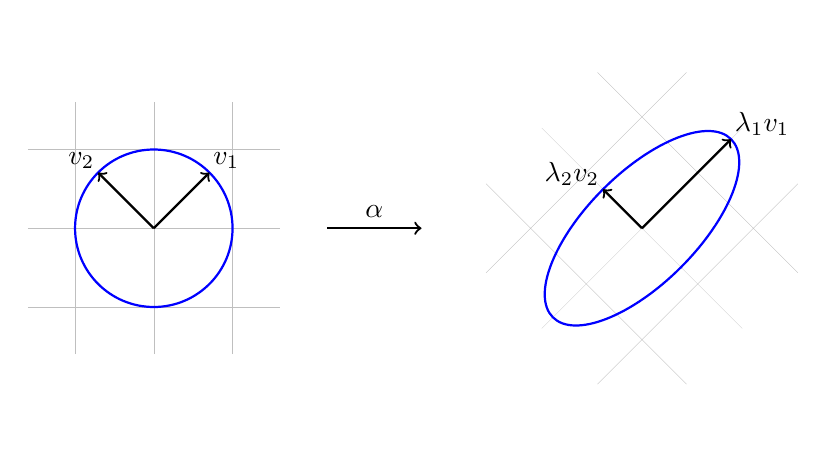
\begin{tikzpicture}[scale=1.0]
    % left: unit circle with eigendirections
    \draw[ultra thin, color=lightgray] (-1.6,-1.6) grid (1.6,1.6);
    \draw[thick, color=blue] (0,0) circle (1);
    \draw[->, thick] (0,0) -- (0.707,0.707) node[above right, inner sep=1pt] {$v_1$};
    \draw[->, thick] (0,0) -- (-0.707,0.707) node[above left, inner sep=1pt] {$v_2$};
    % arrow between
    \draw[->, thick] (2.2,0) -- (3.4,0) node[midway, above] {$\alpha$};
    \begin{scope}[shift={(6.2,0)}, rotate=45]
        \draw[ultra thin, color=lightgray] (-1.8,-1.8) grid (1.8,1.8);
        \draw[thick, color=blue] (0,0) ellipse (1.6 and 0.7);
        \draw[->, thick] (0,0) -- (1.6,0) node[above right, inner sep=1pt] {$\lambda_1 v_1$};
        \draw[->, thick] (0,0) -- (0,0.7) node[above left, inner sep=1pt] {$\lambda_2 v_2$};
    \end{scope}
\end{tikzpicture}
\end{center}

Over $\C$, the same conclusion holds for unitary maps, with almost the same proof.

\begin{lemma}[Eigenvalues of Unitary Maps]
    Let $\alpha$ be a unitary endomorphism of a finite dimensional complex inner product space. Then every eigenvalue of $\alpha$ satisfies $|\lambda| = 1$, and eigenvectors corresponding to distinct eigenvalues are orthogonal.
\end{lemma}
\begin{proof}
    If $\alpha(v) = \lambda v$ with $v \neq 0$, then $\norm{v} = \norm{\alpha(v)} = |\lambda|\norm{v}$, so $|\lambda| = 1$ (in particular $\lambda \neq 0$). If also $\alpha(w) = \mu w$ with $\mu \neq \lambda$, then
    $$
    \lambda\langle v, w \rangle = \langle \alpha(v), w \rangle = \langle v, \alpha^{-1}(w)\rangle = \left\langle v, \tfrac{1}{\mu}w\right\rangle = \frac{1}{\overline{\mu}}\langle v, w\rangle = \mu \langle v, w \rangle,
    $$
    using $\mu\overline{\mu} = 1$, and since $\lambda \neq \mu$ we get $\langle v, w \rangle = 0$.
\end{proof}

\begin{theorem}[Spectral Theorem for Unitary Maps]
    Let $V$ be a finite dimensional complex inner product space, and let $\alpha: V \rightarrow V$ be unitary. Then $V$ has an orthonormal basis of eigenvectors of $\alpha$.
\end{theorem}
\begin{proof}
    As before, we induct on the dimension. Pick an eigenvalue $\lambda$ (which exists as $\F = \C$) with unit eigenvector $v_1$, and let $U = \langle v_1\rangle^\perp$. For $u \in U$,
    $$
    \langle \alpha(u), v_1 \rangle = \langle u, \alpha^{-1}(v_1)\rangle = \left\langle u, \tfrac{1}{\lambda}v_1 \right\rangle = \frac{1}{\overline{\lambda}}\langle u, v_1 \rangle = 0,
    $$
    so $U$ is $\alpha$-stable, and $\alpha|_U$ is a unitary endomorphism of $U$. Induction and the orthogonal decomposition $V = \langle v_1 \rangle \oplus U$ finish the proof as before.
\end{proof}

\begin{remark}
    The restriction to $\C$ really is needed for isometries: the rotation matrix
    $$
    \begin{pmatrix}
        \cos\theta & -\sin\theta \\ \sin\theta & \cos\theta
    \end{pmatrix}
    $$
    is orthogonal, but has eigenvalues $e^{\pm i\theta}$, so is not diagonalisable over $\R$ for general $\theta$ -- there is simply no real direction that a rotation preserves.
\end{remark}

\subsection{Applications to Bilinear Forms}

The spectral theorem lets us sharpen our earlier results on diagonalising symmetric bilinear forms: not only can we diagonalise, we can do so with an \emph{orthonormal} change of basis.

\begin{corollary}[Orthogonal Diagonalisation of Symmetric Matrices]
    Let $A \in \mathcal{M}_{n,n}(\R)$ be symmetric (or $A \in \mathcal{M}_{n,n}(\C)$ Hermitian). Then there is an orthogonal (respectively unitary) matrix $P$ such that $P^TAP$ (respectively $P^\dagger A P$) is diagonal with real entries.
\end{corollary}
\begin{proof}
    View $A$ as a self-adjoint endomorphism of $\F^n$ with the standard inner product. By the spectral theorem there is an orthonormal basis $\{v_1, \dots, v_n\}$ of eigenvectors; let $P$ be the matrix with these as columns. Then $P$ is orthogonal (unitary), and $P^{-1}AP = P^TAP$ (respectively $P^\dagger AP$) is diagonal, with entries the eigenvalues of $A$, which are real.
\end{proof}

Note the happy coincidence that makes this work: for orthogonal matrices, the change of basis formula for linear maps ($P^{-1}AP$) and for bilinear forms ($P^TAP$) \emph{agree}. So the diagonal entries produced are exactly the eigenvalues of $A$, and we can read off the signature of a real symmetric form: $s(\phi) = (\text{number of positive eigenvalues}) - (\text{number of negative eigenvalues})$ of any matrix representing $\phi$.

We can also now prove a satisfying result about pairs of forms.

\begin{corollary}[Simultaneous Diagonalisation of Forms]
    Let $V$ be a finite dimensional real (or complex) vector space, and let $\phi, \psi$ be symmetric (respectively Hermitian) forms on $V$ with $\phi$ positive definite. Then there is a single basis $B$ of $V$ in which $[\phi]_B$ and $[\psi]_B$ are both diagonal.
\end{corollary}
\begin{proof}
    Since $\phi$ is positive definite, it makes $V$ into an inner product space with $\langle u, v\rangle = \phi(u, v)$. By the previous corollary applied in this inner product space, there is a $\phi$-orthonormal basis $B$ of $V$ in which $[\psi]_B$ is diagonal. But orthonormality of $B$ with respect to $\phi$ says precisely that $[\phi]_B = I$, which is certainly diagonal.
\end{proof}

In matrix language: if $A, B$ are real symmetric (or Hermitian) matrices with $A$ positive definite, then there is an invertible $Q$ with $Q^TAQ$ and $Q^TBQ$ both diagonal. This result is the abstract heart of many applications -- for instance, finding the normal modes of a mechanical system simultaneously diagonalises the kinetic and potential energy forms.

And with that, we have reached the end of the course. Starting from nothing but the axioms of a vector space, we have built up bases and dimension, classified linear maps up to change of basis, developed determinants, eigenvalues and canonical forms, and finally seen how an inner product turns linear algebra into geometry. These tools appear constantly throughout mathematics -- and if the subject appeals to you, the story continues in courses on modules (IB Groups, Rings and Modules) and functional analysis, where infinite dimensional spaces take centre stage.

